% \documentclass[a4paper,twoside,11pt]{report}
\documentclass[a4paper,singleside,11pt]{report}

\usepackage{ia_urb_thesis}
\usepackage[italian]{babel}
\usepackage[utf8]{inputenc}
\usepackage[T1]{fontenc}
%\usepackage{lmodern}
\usepackage{amsmath,
	    amsfonts,
	    amstext,
	    amssymb,
	    mathrsfs,
	    stmaryrd,
	    latexsym,
	    %enumitem,
	    % proof,
	    graphicx,
	    epsfig,
	    color,
		caption,
		subcaption,
		textcomp,
		multirow,
	    %hyperref,
	    comment}

\begin{document}

\titolo{Riconoscimento del lavaggio delle \\[5mm]mani tramite smartwatch per ridurre \\[5mm]la trasmissione da contatto di agenti \\[5mm]patogeni}
\candidato{Lorenzo Calisti}
\relatore{Chiar.mo Prof.~Emanuele Lattanzi}
\annoaccademico{2021-2022}

\copertinatesi 
\dedica{Ai miei genitori, a mio zio\\e alle mie nonne.}
\indice
\indicefigure
\indicetabelle
\iniziatesto

\chapter{Introduzione}
\label{cap:introduzione}

Le linee guida della World Health Organization (WHO) indicano che la malattia SARS-CoV-2 coronavirus ed in particolare la sua recente forma COVID-19 si trasmettono principalmente attraverso il contatto corporeo e tramite le goccioline respiratorie (droplets). La trasmissione per contatto avviene quando le mani contaminate toccano le membrane mucose della bocca, del naso o gli occhi. In particolare per quanto riguarda il COVID-19 è stimato che la maggior parte dell'infezione avviene proprio attraverso il contatto delle mani con le superfici contaminate \cite{santarpia2020aerosol}. Per questo motivo una delle misure più importanti che una persona può mettere in pratica per prevenire la trasmissione di germi è prendersi cura dell'igiene delle proprie mani.

Per garantire un'igiene delle mani sufficiente la WHO suggerisce di lavarle accuratamente con acqua e sapone oppure sanificarle utilizzando una sostanza a base di alcool.
Le procedure suggerite in Figura \ref{fig:who-steps} sono composte da molteplici passaggi ciascuno di diversa durata; lavare le mani con acqua e sapone prevede undici step per una durata complessiva fra 
i 40 secondi e i 60 secondi mentre la sanificazione è formata solo da 8 passaggi di durata fra i 20 secondi e i 30 secondi. 
La WHO inoltre indica la sanificazione delle mani con l'alcool come decontaminazione di routine, mentre raccomanda il lavaggio con acqua e sapone solo nei casi in cui le mani sono visibilmente sporche.
Nonostante la provata efficienza di questi due metodi un numero significativo di persone non li mette in pratica a causa della loro difficoltà d'implementazione e si limitano a lavare le loro mani come hanno sempre fatto.

\begin{figure}[!htb]
    \centering
    \begin{subfigure}{.45\textwidth}
        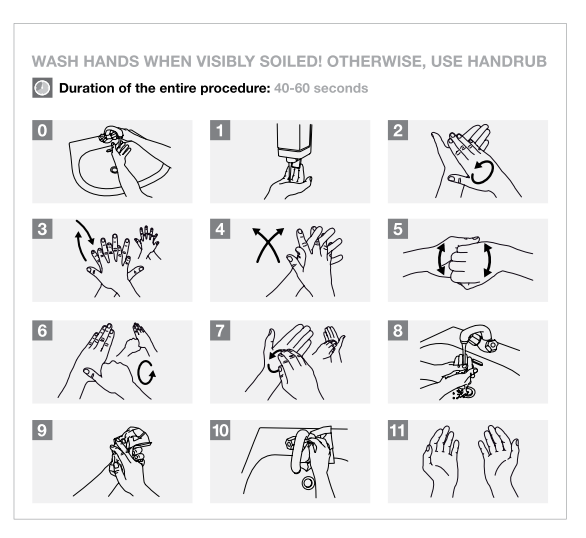
\includegraphics[width=\textwidth]{figure/handwash.png}
        \caption{lavaggio delle mani}
        \label{fig:handwash}
    \end{subfigure}
    \begin{subfigure}{.45\textwidth}
        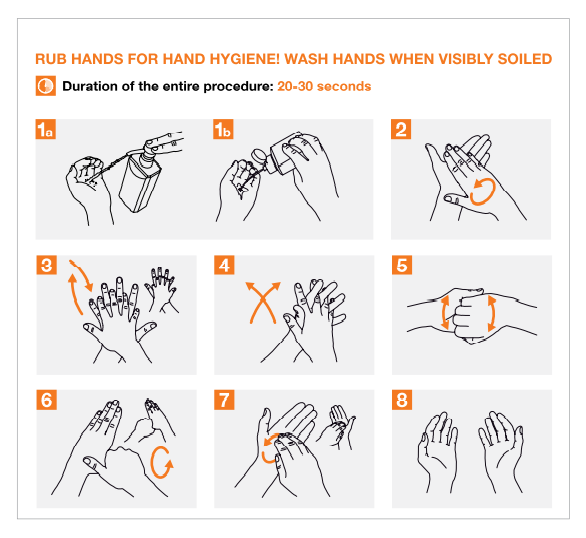
\includegraphics[width=\textwidth]{figure/handsan.png}
        \caption{sanificazione delle mani}
        \label{fig:handsan}
    \end{subfigure}
    \caption{Procedure suggerite dalla WHO per il corretto lavaggio (a) e sanificazione (b) delle mani.}
    \label{fig:who-steps}
\end{figure}

I dispositivi indossabili, come i moderni smartwatch, sono equipaggiati con diversi sensori in grado di misurare continuamente i parametri caratteristici del movimento dei nostri corpi; un esempio è quello di Wang et al.\cite{wang2020accurate} che nel 2020 hanno misurato l'accuratezza di braccialetti indossabili con all'interno accelerometri, giroscopi ed elettrodi per elettromiografia (sEMG) nel identificare e monitorare le procedure di lavaggio e sanificazione delle mani suggerite dalla WHO raggiungendo un'accuratezza superiore al 96\%.
Prima di loro, molti altri autori hanno dimostrato l'efficacia dei dispositivi indossabili nel classificare attività umane generali come ad esempio la corsa, la camminata, salire o scendere le scale, saltare e sedersi\cite{zhang2013human}\cite{sztyler2016body}\cite{sztyler2017position}\cite{bhat2018online}\cite{koping2018general}\cite{lattanzi2022exploring}.

La facile reperibilità di data-set di grandi dimensioni per il riconoscimento di attività umane, assieme ai recenti sviluppi nel deep learning, hanno portato ad incredibili risultati aumentando significativamente l'accuratezza nella classificazione delle attività generali che ora raggiunge anche valori del 99\%\cite{cheng2010active}\cite{singh2017convolutional}\cite{hassan2018robust}\cite{hou2020study}.

Quando non si seguono le procedure raccomandate dalla WHO l'attività di lavare le mani è eseguita in maniera molto personale il che ci porta ad ottenere dei dati che definiamo completamente non strutturati.
Questi dati non strutturati, assieme alle strabilianti performance ottenute dai sistemi di machine learning e alla facilità nel reperire data-set di grandi dimensioni porta alla nascita di nuovi problemi
etici che non possono essere trascurati \cite{muller2021ten}. Inoltre, a differenza delle attività che coinvolgono l'intero corpo, come la camminata o la corsa, lavare le mani richiede movimenti molto precisi di muscoli, tendini e ossa delle dita che non è scontato siano facilmente riconoscibili a partire da dati raccolti, dal polso del soggetto tramite un comune smartwatch. 

Per i motivi sopra citati in questa tesi ci concentreremo sul riconoscimento dei lavaggi/sanificazioni delle mani partendo da dati non strutturati con lo scopo di investigare l'accuratezza nella 
classificazione di un sistema basato su smartwatch capace di monitorare l'igiene delle mani nella gran parte della popolazione. In particolare, in questa tesi, introduciamo uno studio sperimentale 
estensivo volto a valutare l'abilità di un sistema di machine learning automatico di distinguere i gesti di lavaggio e sanificazione dal resto delle attività che ogni persona compie giornalmente 
senza l'utilizzo di strumenti invasivi, ma facendo affidamento solo su dispositivi indossabili comuni come smartwatch disponibili commercialmente.

Nei capitoli seguenti di parlerà in maniera più approfondita dei sistemi di machine learning presi in esame descrivendo lo stato dell'arte in questo ambito ed illustrando i metodi e le relative scelte fatte 
durante lo svolgimento della ricerca e presentando i risultati della valutazione sperimentale dei diversi modelli sia su PC che sul dispositivo embedded utilizzato come benchmark: l'HEXIWEAR. Infine si presenterà lo sviluppo di un'applicazione per il monitoraggio dell'igiene delle mani creata per lo smartwatch HEXIWEAR e che fa largo utilizzo dei modelli d machine learning per il riconoscimento degli eventi.
\chapter{Background}
\label{cap:background}

\section{Stato dell'arte}
\label{sec:stato-dell-arte}

Al momento della scrittura di questa tesi non sono stati trovati dispositivi validati scientificamente in grado di riconoscere le attività di lavaggio e sanificazione delle mani tramite comuni strumenti indossabili. L'unico sistema disponibile commercialmente è SureWash, prodotto dalla GLANTA Ltd, che è in grado di riconoscere i movimenti delle mani dello staff di un ospedale partendo da dati video, ma è limitato al solo riconoscimento di alcuni degli step suggeriti dalla WHO.
Il rilevamento dei movimenti delle mani utilizzando sistemi video è stato studiato da diversi autori, per esempio Zhong et al. nel 2020 hanno proposto un sistema multi-camera in grado di riconoscere sette azioni specifiche legate all'igiene delle mani\cite{zhong2020multi}; più recentemente, Yue et al. sono stati in grado di identificare correttamente sette passaggi del metodo prescritto da alcuni ospedali utilizzando uno strumento di machine learning pre-addestrato chiamato YOLO v3\cite{yue2021intelligent}.
Purtroppo uno dei problemi più grandi di questi sistemi è la privacy, per funzionare infatti richiedono l'installazione di molteplici videocamere in diverse stanze.

Un approccio ortogonale si concentra sul riconoscimento delle attività di lavaggio delle mani tramite sensori inerziali (IMU). In questo ambito è presente un numero ridotto di contributi scientifici, molti dei quali si basano sull'utilizzo di molteplici sensori ad alta sensitività e accuratezza, tipici degli strumenti scientifici\cite{galluzzi2015hand}\cite{bal2017system}\cite{li2018wristwash}. 
Anche se le IMU non acquisiscono dati video è comunque importante tenere in considerazione i problemi di privacy, infatti, molti autori hanno mostrato come sia possibile estrarre informazioni chiave riguardanti l'identità dell'utilizzatore partendo dai dati non processati degli accelerometri\cite{jain2018gender}\cite{van2019systematic}.

Queste ricerche preliminari mostrano che il riconoscimento automatico delle attività di lavaggio delle mani attraverso sensori inerziali (accelerometro e giroscopio) è possibile, ma, non approfondiscono le potenzialità degli smartwatch disponibili commercialmente e nemmeno l'applicazione di tecniche di deep learning moderne.

A partire dal 2015 ad oggi sono stati pubblicati solo alcuni lavori rilevanti che fanno uso di smartwatch commerciali: il primo, presentato da Moldol et al., descrive un sistema di monitoraggio in grado di interagire con un distributore di sapone smart per riconoscere l'inizio della procedura di lavaggio\cite{mondol2015harmony}; nel 2020, Mondol et al. e Banerjee et al. hanno presentato due soluzioni per verificare la conformità delle norme della WHO partendo da segnali di sensori IMU \cite{mondol2020hawad}\cite{banerjee2020hand}; più recentemente, Samyoun et al. hanno presentato un sistema di valutazione del lavaggio delle mani basato su smartphone\cite{samyoun2021iwash}, mentre nel 2021, Wu et al. hanno presentato un sistema autonomo di monitoraggio combinando diverse tecnologie di IoT con videocamere e smart dispenser in grado di dare all'utente feedback sul processo di lavaggio delle mani. Infine nel 2022 Fagert et al. hanno introdotto una nuova modalità di rilevamento del lavaggio delle mani misurando le vibrazioni indotte dall'attività sulla struttura del lavandino\cite{fagert2022clean}.

\section{Algoritmi di Machine Learning}
\label{sec:algoritmi-di-machine-learning}

In questa sezione parliamo in maniera più approfondita degli strumenti di apprendimento automatico presi in esame; in particolare per quanto riguarda gli strumenti di machine learning standard abbiamo valutato la Support Vector Machine (SVM) e l'Ensemble Subspace con K-Nearest Neighbors (ES-KNN), mentre nel campo del deep learning abbiamo considerato una Rete Neurale Convoluzionale (CNN) ed un Long Short-Term Memory (LSTM).

\subsection{Support Vector Machine (SVM)}
\label{ssec:support-vector-machine}

SVM è uno degli algoritmi di machine learning più semplici e più utilizzati tradizionalmente per i problemi di regressione e di classificazione con un numero ridotto di campioni.
Un modello SVM rappresenta i dati in input come dei punti nello spazio, mappati in modo tale che i dati appartenenti alle diverse classi siano separati da un margine ampio. I dati sconosciuti sono inseriti nello stesso spazio e la loro categoria dipende dalla regione in cui cadono.

Formalmente, una SVM costruisce un iperpiano, o un insieme di iperpiani, Figura \ref{fig:svm}, in uno spazio a più dimensioni; intuitivamente una buona separazione si può ottenere dall'iperpiano con la distanza maggiore dal punto del training set più vicino di ognuna delle classi; in generale maggiore è il margine fra questi punti, minore è l'errore di generalizzazione commesso dal classificatore. 

Spesso capita che gli insiemi da distinguere non siano linearmente separabili nello spazio, per questo motivo si tende a mappare lo spazio originale in uno con un numero di dimensioni maggiore attraverso funzioni che vengono definite kernel scelte in base al problema da risolvere.

In questa tesi si è optato per l'utilizzo di un SVM con kernel polinomiale, anche se altri kernel sono stati valutati (lineare, quadratico e gaussiano), ma non hanno raggiunto le sue performance.

\begin{figure}[!htb]
    \centering
    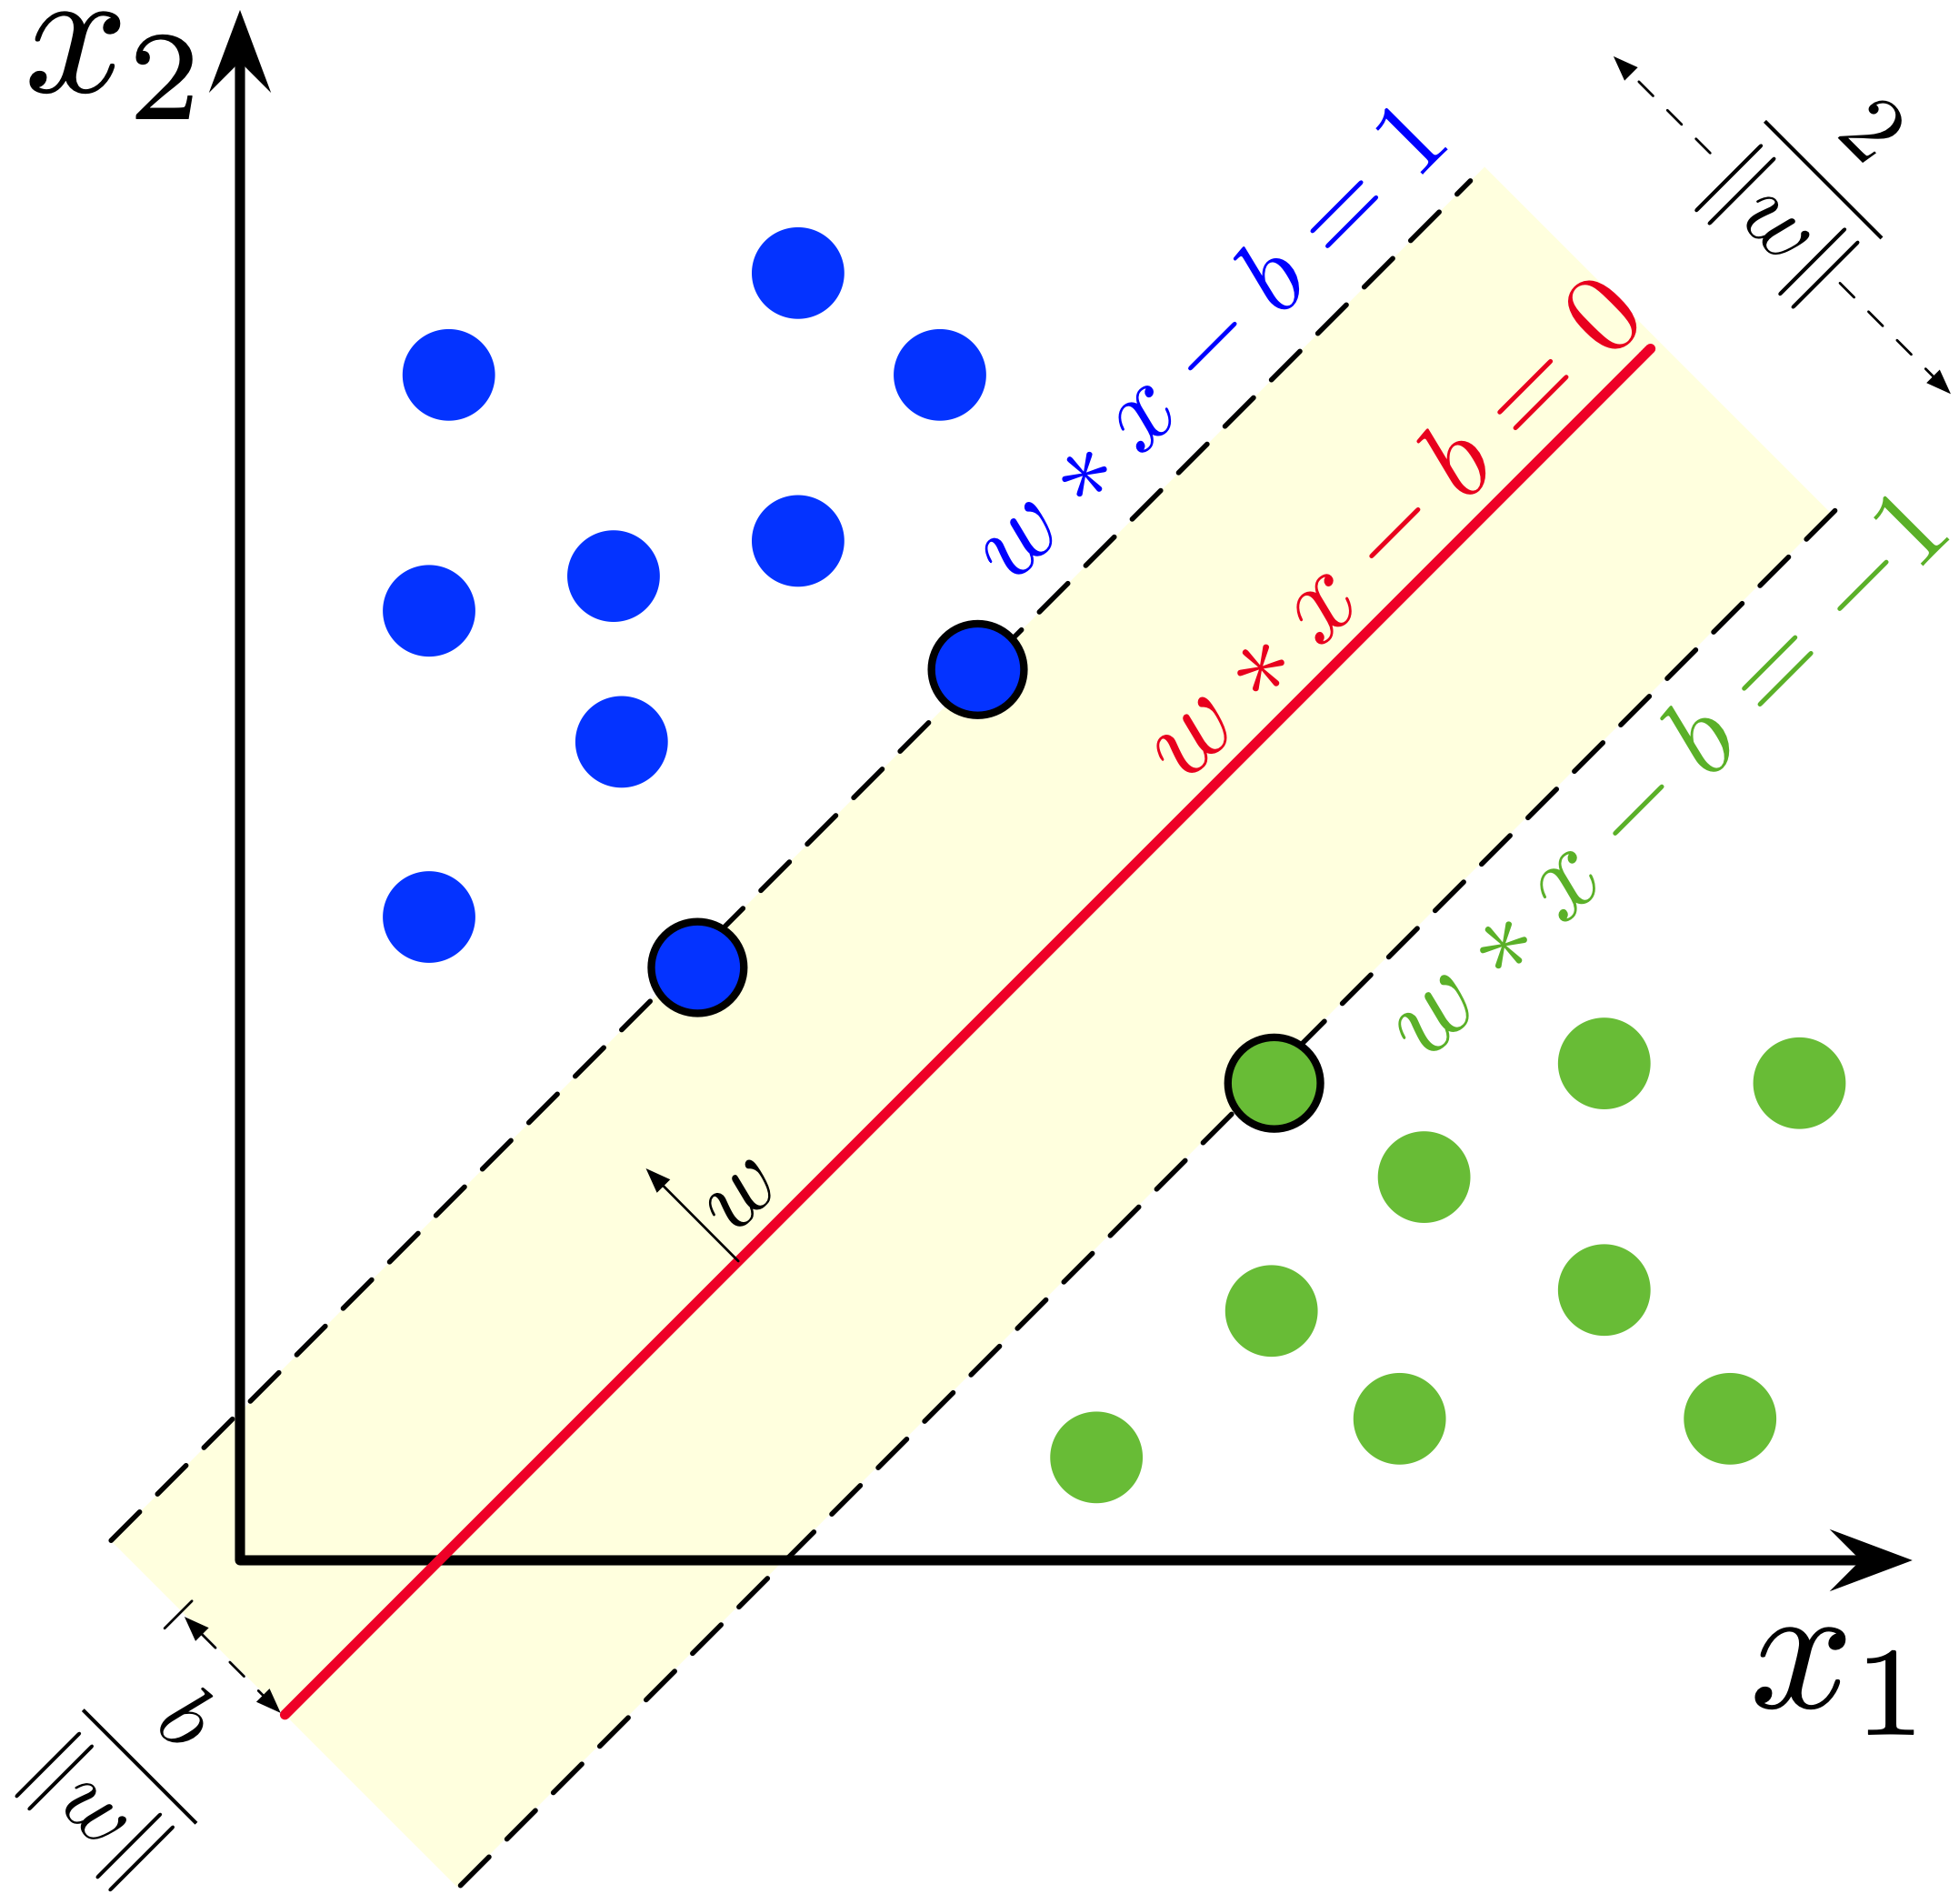
\includegraphics[width=.4\textwidth]{figure/svm.png}
    \caption{Esempio d'iperpiano che meglio separa le due classi di un SVM con kernel lineare.}
    \label{fig:svm}
\end{figure}

\subsection{Ensemble Subspace con K-Nearest Neighbors (ES-KNN)}
\label{ssec:ensemble-subspace-con-knn}

K-Nearest Neighbors (KNN) è un'altro algoritmo di apprendimento automatico molto utilizzato per le sue prestazioni e semplicità. L'algoritmo sfrutta una metrica di distanza per assegnare ad un dato ignoto una classe in base alla maggioranza dei voti dei suoi k vicini. Il parametro k è un intero positivo non molto grande, se k=1 allora l'oggetto viene assegnato alla classe del suo vicino. 

Lo spazio viene partizionato in regioni in base alle posizioni e alle caratteristiche degli oggetti di apprendimento (Figura \ref{fig:knn}), ai fini del calcolo della distanza gli oggetti sono rappresentati attraverso vettori in uno spazio multidimensionale, spesso si usa la distanza euclidea, ma anche altri tipi di distanza sono ugualmente utilizzabili, ad esempio la distanza Manhattan. 
Un punto è assegnato alla classe C se questa è la più frequente fra i k esempi più vicini all'oggetto sotto esame, i vicini sono presi da un insieme di oggetti per cui è nota la classificazione corretta. 

Nonostante la sua semplicità, KNN offre dei risultati competitivi, e in alcuni casi supera di gran lunga altri complessi algoritmi d'apprendimento. Per migliorare le performance di classificazione del KNN nella letteratura sono state proposte delle tecniche di ensemble. In generale le tecniche di ensemble consistono nell'addestrare molteplici modelli per poi combinarli assieme, ad esempio facendo la media, per ottenere l'output desiderato. Un modo per creare un ensemble è quello di addestrare i classificatori con dataset differenti ottenuti suddividendo il training set originario; 
questa tecnica è nota come ensemble subspace. In questa tesi ci concentriamo su una classe di ensemble subspace nota come Ensemble Random Subspace KNN (ERS-KNN) per cui il training set è suddiviso randomicamente nei subspace.

\begin{figure}[!htb]
    \centering
    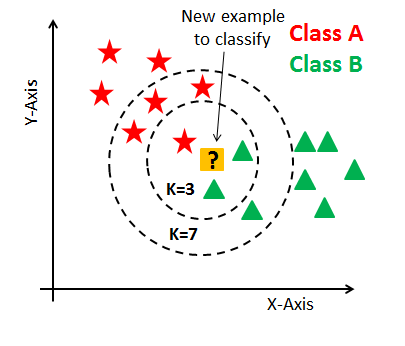
\includegraphics[width=.5\textwidth]{figure/knn.png}
    \caption{Esempio di classificazione di un nuovo dato in un modello KNN binario.}
    \label{fig:knn}
\end{figure}

\subsection{Convolutional Neural Network (CNN)}
\label{ssec:convolutional-neural-network}

CNN(Figura \ref{fig:cnn}) è uno strumento di classificazione dei dati che appartiene alla categoria del deep learning, molto utilizzato negli ultimi anni grazie alla sua struttura che segue un approccio basato sulla computer vision facendo uso delle informazioni spaziali e temporali ricavate dai dati. La struttura della CNN è ispirata dai processi biologici che avvengono nella corteccia visiva degli animali, i cui neuroni sono disposti in maniera tale da rispondere alle regioni di sovrapposizione che tassellano il campo visivo.

Nella pratica CNN è un'estensione di un Multi-Layer Perceptron composto da uno strato di input, vari strati convoluzionali, di pooling e densamente connessi fra loro. Lo strato di input ha il compito di raccogliere i dati sotto forma di pixel di un'immagine e passarli agli strati successivi; i livelli convoluzionali sono il nucleo della rete e contengono diversi kernel che convolgono con i dati di input. La convoluzione estrae automaticamente le feature più significative dai dati riducendo la dimensionalità, inoltre l'aggiunta di strati di pooling aiuta a ridurre ulteriormente la dimensione dei parametri andando a fare sub-sampling. Infine uno o più livelli densamente connessi si comportano come un Perceptron tradizionale prendendo le feature in input e producendo una classe in output.

\begin{figure}[!htb]
    \centering
    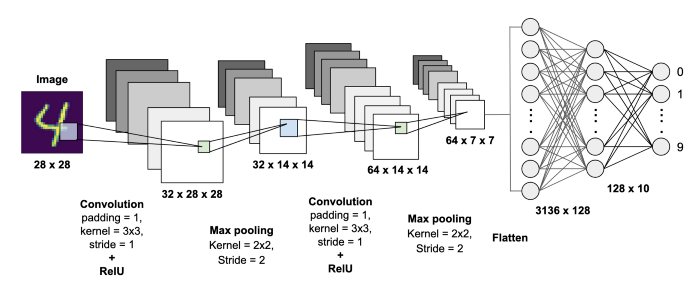
\includegraphics[width=\textwidth]{figure/cnn.png}
    \caption{Esempio della struttura di una rete CNN.}
    \label{fig:cnn}
\end{figure}

\subsection{Long Short-Term Memory (LSTM)}
\label{ssec:long-short-term-memory}

LSTM è una variante delle Reti Neurali Ricorrenti (RNN) utilizzata nel campo del deep learning e dell'intelligenza artificiale per la sua abilità nel classificare e fare predizioni basandosi sui dati delle serie temporali; per questo motivo è spesso usata in ambiti come il riconoscimento della scrittura, il riconoscimento del parlato, la traduzione di testi, il controllo di robot e le applicazioni sanitarie.

Un'unità LSTM(Figura \ref{fig:lstm}) è composta da una cella, un gate di input, un gate di output ed un forget gate; la cella ricorda valori per un tempo arbitrario, mentre i tre gate regolano il flusso delle informazioni dentro e fuori dalla cella prendendo decisioni su cosa ricordare e cosa dimenticare. Il nome LSTM si riferisce al fatto che questo modello ha sia una memoria a lungo termine che una a breve termine, analoga alla struttura del cervello umano.

\begin{figure}[!htb]
    \centering
    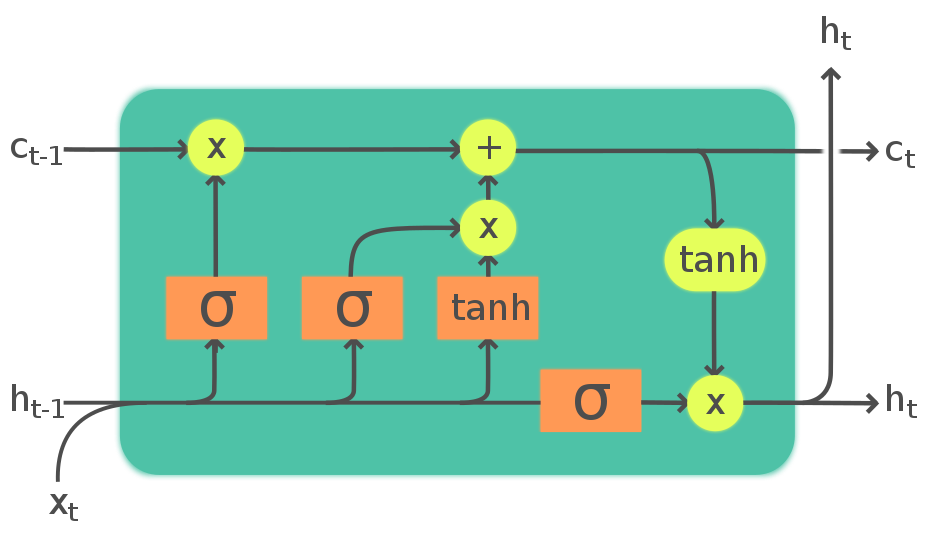
\includegraphics[width=.5\textwidth]{figure/lstm.png}
    \caption{Esempio di una singola unità di una rete LSTM.}
    \label{fig:lstm}
\end{figure}

\section{L'HEXIWEAR}
\label{sec:hexiwear}

Lo smartwatch utilizzato durante la ricerca è l’HEXIWEAR progettato da MikroElektronika in collaborazione con NXP. HEXIWEAR (Figura \ref{fig:hexiwear}) è uno smartwatch completamente open-source dal costo di circa 50\$ che consente lo sviluppo di applicazioni IoT in maniera molto semplice; al suo interno monta ben due MCU: la prima è una Kinetis K64F con architettura ARM Cortex-M4, una frequenza massima di 120MHz, 1024KB di memoria Flash e 256KB di memoria RAM; la seconda è un SoC Kinetis KW40z che permette l’utilizzo delle funzionalità Bluetooth Low Energy. 
All'interno dell'HEXIWEAR sono inoltre presenti una grande quantità di sensori integrati, come ad esempio: 

\begin{itemize}
    \item accelerometro e magnetometro a sei assi FXOS8700
    \item giroscopio a tre assi FXAS21002
    \item sensore di altitudine e pressione MPL3115A2
    \item sensore di temperatura ed umidità HTU21D
    \item sensore di luminosità TSL2561
    \item sensore per il rilevamento dei battiti cardiaci MAX30101
\end{itemize}

Inoltre sono presenti anche un display OLED da 1.1 pollici, una batteria ricaricabile Li-Po da 190mAh e diverse interfacce come: USB, UART, SPI, I2C e SD-card.
Per facilitare lo sviluppo ed il debug delle applicazioni HEXIWEAR ha una docking station al quale è possibile connettere lo smartwatch ed estendere le sue feature con oltre 200 apposite schede dette click boards.

Per sviluppare le applicazioni nell'HEXIWEAR si è deciso di utilizzare la piattaforma MbedOS. Mbed è un sistema operativo real-time open-source creato da ARM per i dispositivi embedded con memoria limitata e che richiedono un basso consumo di corrente. 
Mbed fornisce agli sviluppatori un livello di astrazione tramite il quale possono creare applicazioni IoT scrivendole direttamente in C/C++; esso consiste in un insieme di librerie che forniscono i driver per le periferiche del micro-controllore, l'accesso alla rete, il controllo dell'ambiente RTOS, gli strumenti di build e degli script per test e debug, inoltre è disponibile una repository online dalla quale é possibile scaricare librerie esterne create dalla community.

\begin{figure}[!htb]
    \centering
    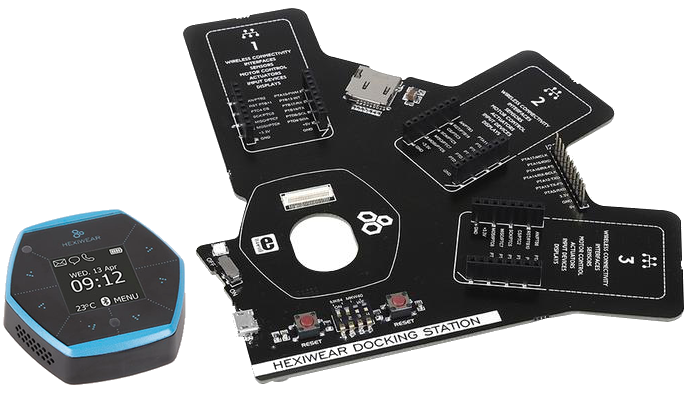
\includegraphics[width=.8\textwidth]{figure/hexiwear.png}
    \caption{HEXIWEAR e la sua docking station.}
    \label{fig:hexiwear}
\end{figure}
\chapter{Metodi}
\label{cap:metodi}

\section{I dataset}
\label{sec:dataset}

Prima di poter valutare l'accuratezza dei modelli di machine learning proposti è necessario addestrarli con un apposito dataset; in questa tesi i modelli sono stati valutati utilizzandone due: uno creato ad hoc per questa tesi ed il Daily Living Activities (DLA) disponibile pubblicamente\cite{leotta2021daily}.

Al momento della ricerca non sono disponibili dataset pubblici contenenti dati di lavaggi e sanificazioni delle mani mediante segnali di accelerometro e giroscopio; per questo motivo si è deciso di crearne uno personalizzato raccogliendo i dati da una Inertial Measurement Unit (IMU) posizionata sul polso della mano dominante di quattro partecipanti durante attività di vita reale.

Per raccogliere i dati abbiamo utilizzato una IMU Shimmer3 equipaggiata con un accelerometro e un giroscopio tri-assale\cite{shimmer}; questo dispositivo, visibile in Figura \ref{fig:shimmer}, è progettato appositamente per essere indossato ed è spesso utilizzato nel monitoraggio delle attività nell'ambito delle scienze sportive e mediche. Al suo interno monta una serie di sensori wide-range con campionamento a 14 bit, range da $\pm2.0g$ fino a $\pm16.0g$ ed una sensitività da $1mg/LSB$ fino a $12mg/LSB$; lo Shimmer3 può essere considerato una buona rappresentazione delle IMU correntemente equipaggiate all'interno degli smartwatch commerciali. Il dispositivo indossabile è stato programmato per campionare il suo accelerometro e giroscopio ad una frequenza di 100Hz e salvare i dati raccolti in una SD-card interna. Per rimuovere il bias dei sensori il dispositivo è stato calibrato all'inizio della ricerca lasciandolo su una superficie piana per circa 30 secondi in modo da ottenere una traccia di calibrazione.
In Figura \ref{fig:acc-gyro-plot} vediamo un'esempio delle sei tracce di accelerometro e giroscopio raccolte durante un'attività di sanificazione delle mani.

\begin{figure}[!htb]
    \centering
    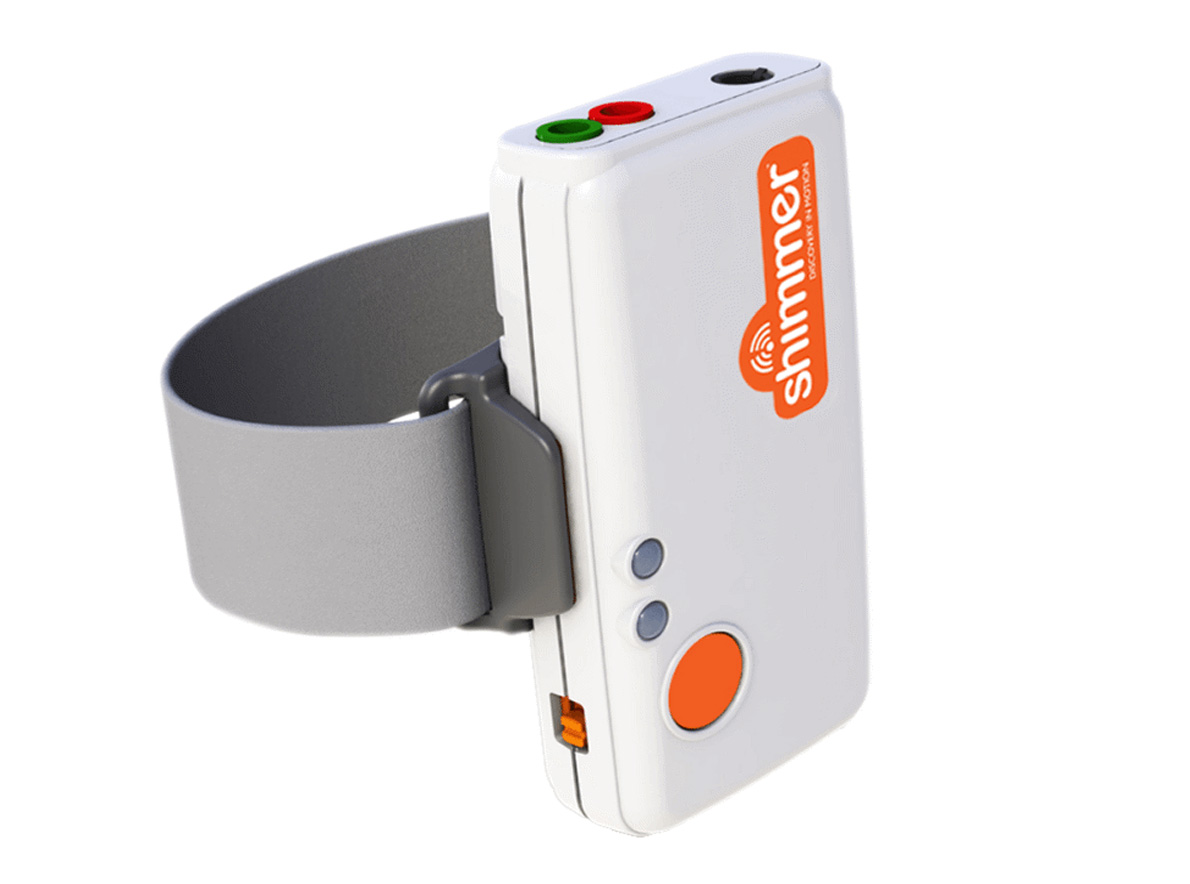
\includegraphics[width=.4\textwidth]{figure/shimmer.jpg}
    \caption{IMU Shimmer3 dotata di bracciale per essere indossata al polso dell'utente.}
    \label{fig:shimmer}
\end{figure}

\begin{figure}[!htb]
    \centering
    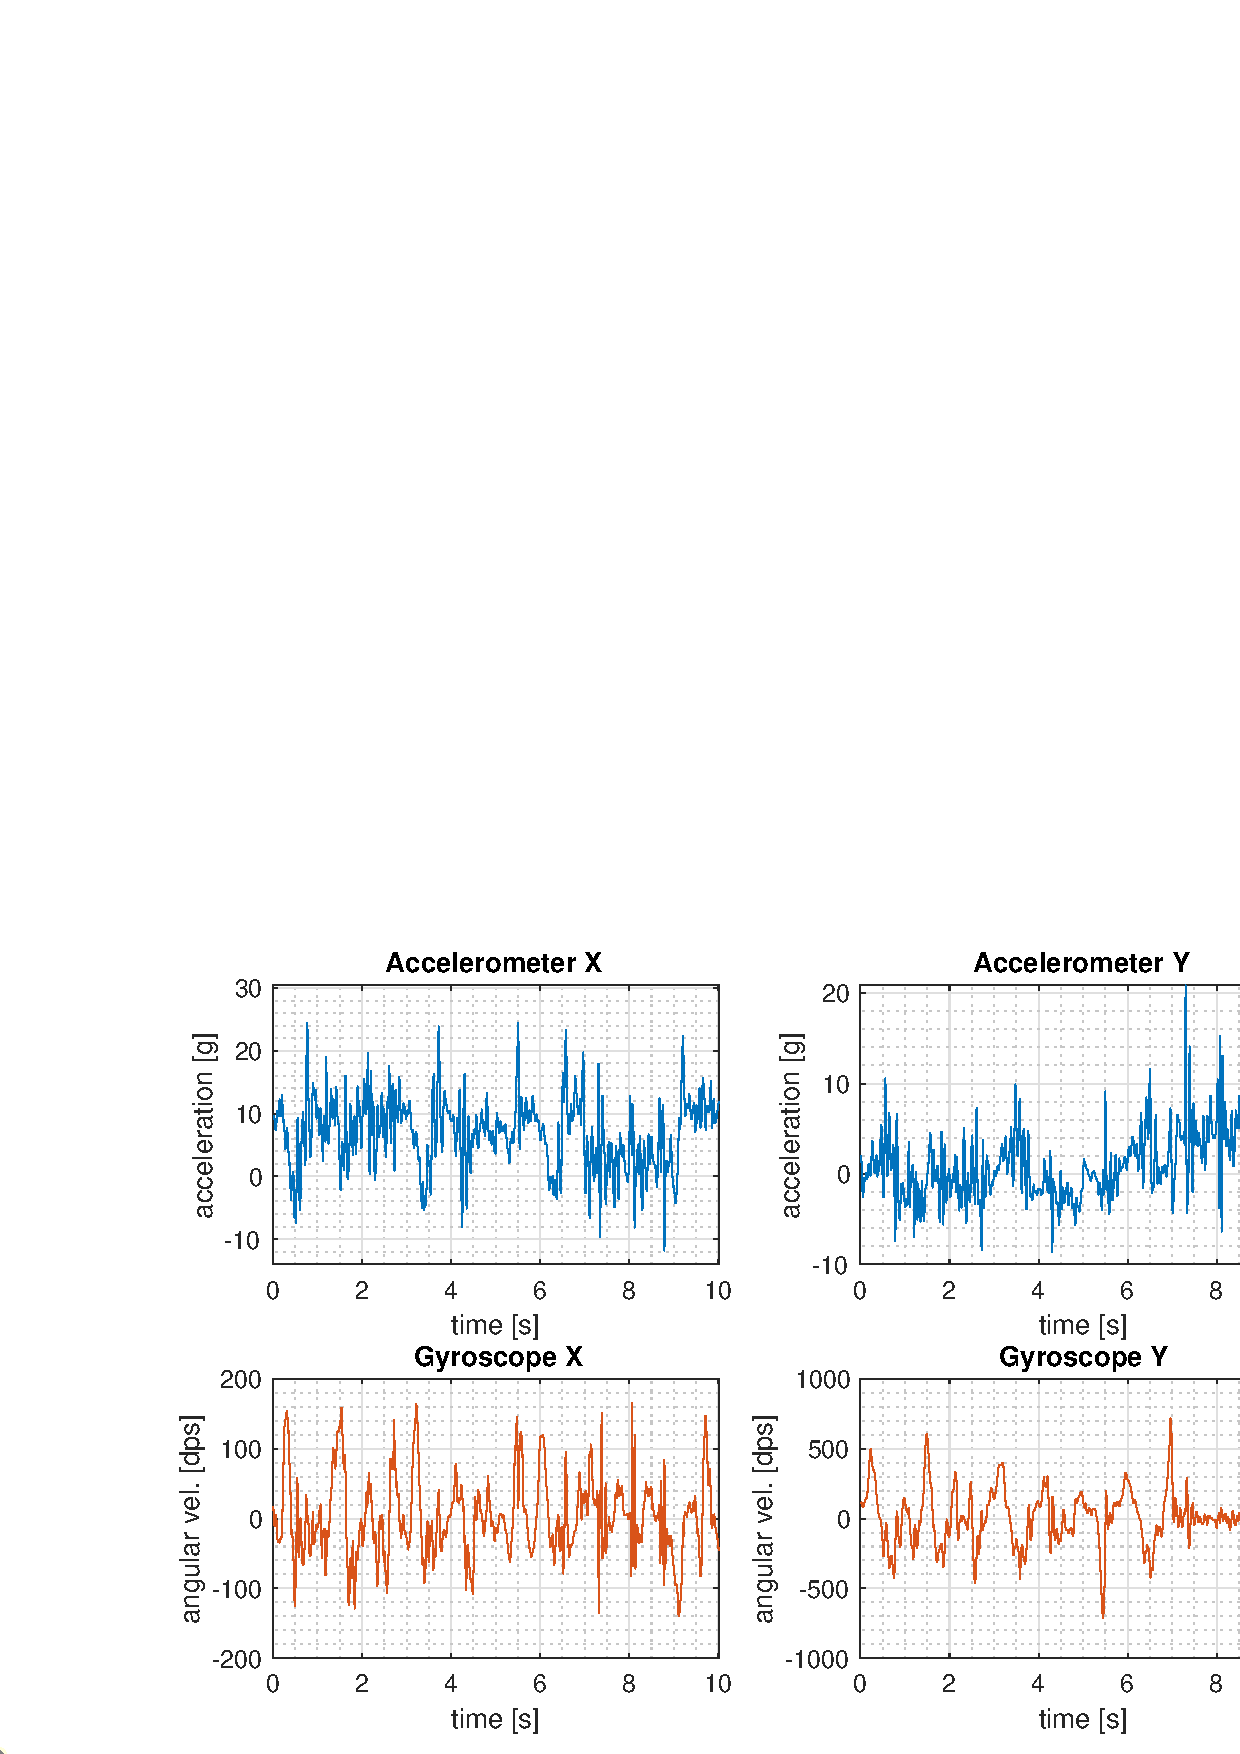
\includegraphics[width=\textwidth]{figure/acc_gyr_plot.pdf}
    \caption{Tracce di accelerometro e giroscopio prodotte durante un'attività di sanificazione delle mani.}
    \label{fig:acc-gyro-plot}
\end{figure}

\`E importante notare che i soggetti non sono istruiti sulla corretta maniera in cui lavare o sanificare le mani e sono stati lasciati completamente liberi di usare il loro metodo abituale in modo da raccogliere dati il più possibile non strutturati. La Tabella \ref{tab:activity-duration} mostra la durata media e la deviazione standard degli eventi di lavaggio e sanificazione per ognuno dei quattro soggetti assieme ad una media e deviazione standard cumulativa. Come si può notare la durata media dipende significativamente dal soggetto.

\begin{table}
    \centering
    \begin{tabular}{c c c}
        \hline
        soggetto & lavaggi & sanificazioni  \\
        \hline
        0 & $66.68s \pm 18.69s$ & $23.66s \pm 6.26s$  \\
        1 & $31.92s \pm 8.97s$  & $26.09s \pm 3.67s$  \\
        2 & $39.47s \pm 8.52s$  & $19.18s \pm 4.29s$  \\
        3 & $30.54s \pm 6.17s$  & $25.44s \pm 8.59s$ \\
        \hline
        media & $50.92 \pm 22.29s$  & $23.59 \pm 7.33s$ \\
        \hline
    \end{tabular}
    \caption{Durata delle attività registrate dal dataset ad hoc in secondi.}
    \label{tab:activity-duration}
\end{table}

Il secondo dataset preso in considerazione è il Daily Living Activities (DLA) che è uno dei pochi dataset disponibili contenente dati di lavaggi di mani campionati attraverso sensori inerziali. Questo dataset è stato creato registrando diverse parti del corpo ed utilizzando differenti sensori indossabili; in particolare dal polso, dai fianchi e dalle caviglie di otto volontari in salute con età compresa fra i 23 e i 37 anni. Il dataset è composto da 17 differenti attività di uso comune, ma, poiché il nostro scopo è valutare i lavaggi delle mani abbiamo filtrato solo i dati raccolti dal polso e rimosso tutte quelle azioni che non hanno a che vedere con le mani. In questo dataset non sono presenti dati raccolti durante la sanificazione, inoltre i sensori utilizzati per la raccolta non sono equipaggiati con un giroscopio il chè può sembrare svantaggioso, ma ci consente di soppesare l'utilità dei segnali del giroscopio e di valutare l'abilità dei modelli proposti nel generalizzare.

\section{Le finestre di campionamento}
\label{sec:le-finestre-di-campionamento}

Le tracce raccolte dal dataset costruito ad hoc sono composte da sei segnali distinti, tre per l'accelerometro e tre per il giroscopio, mentre quelle del dataset DLA hanno solo tre tracce per l'accelerometro; in entrambi i casi le tracce sono state suddivise in finestre ognuna delle quali è considerata come un campione da usare per l'addestramento dei modelli. Ogni campione è stato etichettato durante la fase di raccolta dei dati marchiandolo con un'etichetta che rappresenta il soggetto ed una che rappresenta la categoria di azione compiuta fra queste: lavaggio, sanificazione, altro.

Decidere la dimensione della finestra è un'operazione non semplice poiché influisce sulle performance dei modelli in molti modi diversi; infatti, dev'essere larga abbastanza per includere informazioni significative sulla singola attività, ma non dev'essere troppo grande da includere multipli eventi successivi. Nell'ambito del riconoscimento delle attività umane sono state utilizzate finestre di diversa lunghezza, da 1 secondo fino a 30 secondi\cite{cheng2010active}\cite{hassan2018robust}; in alcuni casi si è arrivati addirittura a finestre piccolissime (solo 0.06 secondi) con un overlap del 70\% fra di loro in modo da riconoscere ogni passaggio della procedura strutturata.

In questa ricerca non dovendoci preoccupare del riconoscimento di dati strutturati abbiamo valutato finestre di dimensione maggiore: dai 2 secondi fino ai 20 secondi e senza overlap fra le finestre. Inoltre, a causa del protocollo di raccolta dei dati proposto, che punta a campionare continuamente i sensori, il numero di altri eventi rispetto ai lavaggio/sanificazioni è di gran lunga maggiore, per questo motivo i campioni etichettati come altro sono stati randomicamente selezionati e ridotti di numero per ri-bilanciare il dataset.

\section{I Classificatori}
\label{sec:classificatori}

Per addestrare e testare l'accuratezza dei modelli di machine learning tradizionali i segnali in input devono essere processati in modo da estrarre una serie di feature significative; in questo lavoro abbiamo delineato tre tipologie di feature. La prima categoria è composta dalle feature Base, ovvero dei descrittori statistici classici come:

\begin{enumerate}
    \item media
    \item deviazione standard
    \item massimo e minimo
    \item mediana
\end{enumerate}

i quali descrivono la tendenza dei campioni, la seconda categoria è quella delle feature Hjorth formata da:

\begin{enumerate}
    \item attività
    \item mobilità
    \item complessità
\end{enumerate}

che catturano le caratteristiche principali del segnale nel dominio della frequenza rappresentando la potenza del segnale e la sua frequenza media, mentre la terza categoria è quella delle feature Shape formata da:

\begin{enumerate}
    \item curtosi 
    \item skewness
\end{enumerate}

con l'obbiettivo di descrivere la forma dei dati, ovvero quanto i dati in esame si discostano da una distribuzione normale.

Nel caso degli approcci di deep learning non è necessario eseguire l'estrazione delle feature utilizzando direttamente i campioni dei segnali divisi in finestre come input della classificazione. Per quanto riguarda la CNN, che comunemente è applicata all'analisi delle immagini, è necessario un passaggio di preprocessing che converte i dati delle serie temporali in un formato visuale. Questa possibilità ha recentemente attratto grande attenzione in letteratura portando alla nascita di diverse strategie di conversione; in questo studio ci concentriamo su un metodo che codifica i dati delle serie temporali in immagini chiamato Gramian Angular Summation/Difference Field(GASF, GADF)\cite{wang2015imaging}. Questo metodo rappresenta le serie temporali in un sistema di coordinate polari, invece delle tipiche coordinate Cartesiane, con il vantaggio di mantenere intatte le relazioni spaziali e temporali. 

Poiché questo approccio porta ad avere due immagini per asse, una per il Gramian Angular Summation(GASF) e l'altra per il Gramian Angular Difference(GADF), nel caso del dataset ad hoc otteniamo un set di 12 immagini, mentre nel caso del dataset DLA solo 6; di conseguenza il modello CNN(Figura \ref{fig:models:cnn}) prende come input un'immagine quadrata a 12 o 6 canali costruita a partire dai dati della finestra e la cui altezza e larghezza dipendono dalla dimensione della finestra (WS). L'immagine è quindi convoluta attraverso quattro livelli convoluzionali di dimensione decrescente intermezzati da livelli di normalizzazione, ReLu e max pooling che hanno l'effetto di stabilizzare il processo di apprendimento diminuendo il numero di epoche richieste. L'output è poi passato attraverso tre livelli densamente connessi ed un Softmax che hanno lo scopo di assegnare ad ogni classe una probabilità proporzionale al segnale di output.

\begin{figure}[!htb]
    \centering
    \begin{subfigure}{\textwidth}
        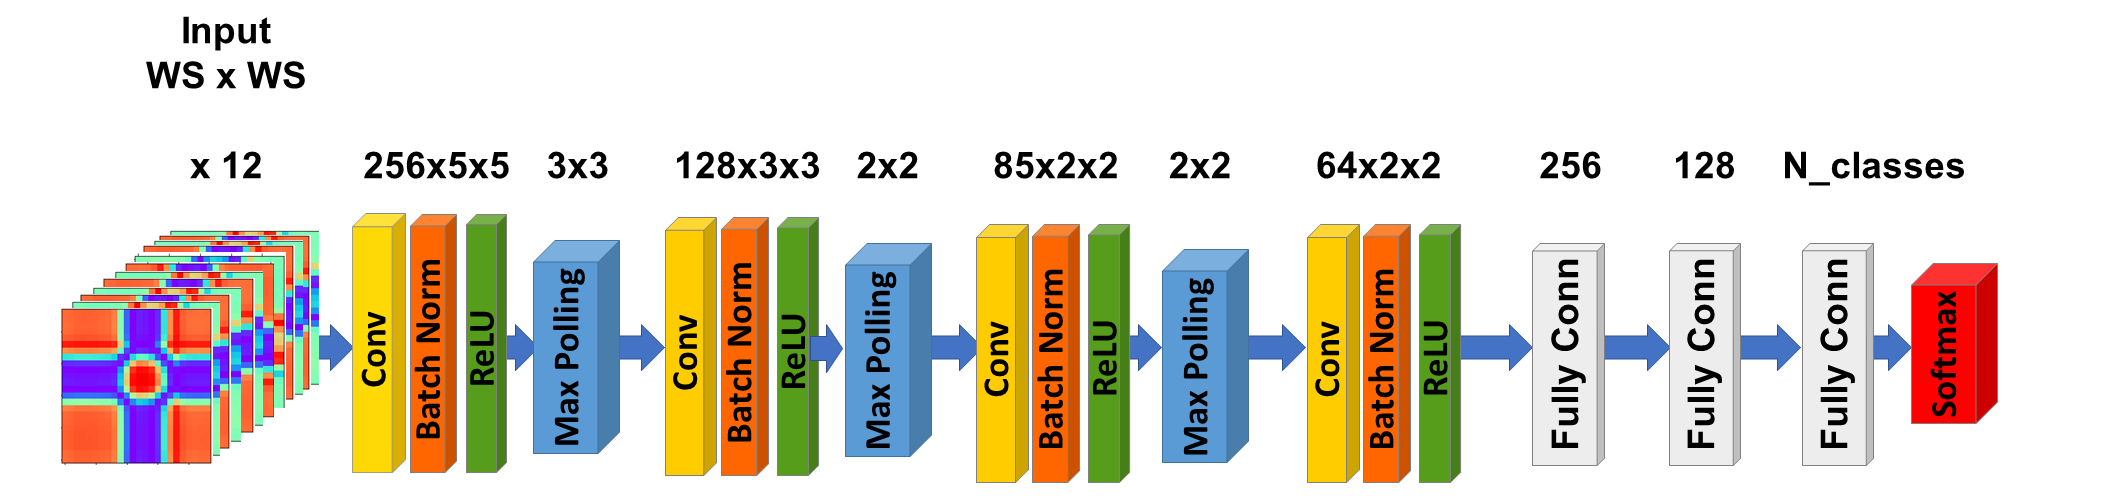
\includegraphics[width=\textwidth]{figure/cnn_model.png}
        \caption{architettura del modello CNN}
        \label{fig:models:cnn}
    \end{subfigure}
    \begin{subfigure}{\textwidth}
        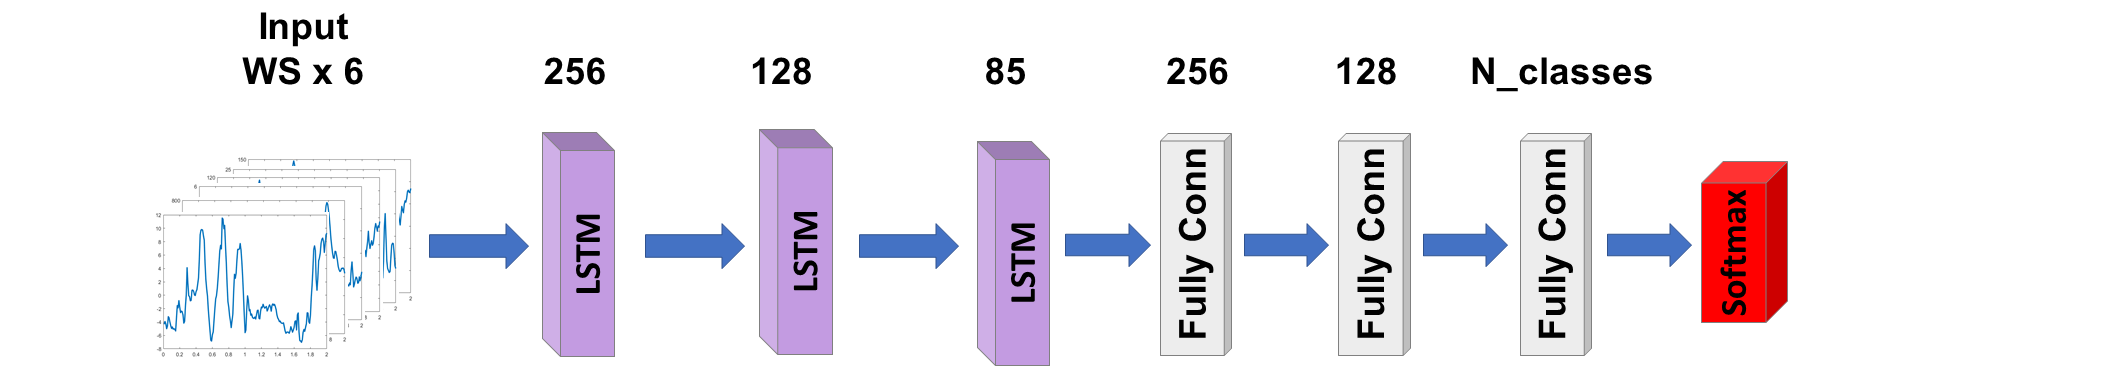
\includegraphics[width=\textwidth]{figure/lstm_model.png}
        \caption{architettura del modello LSTM}
        \label{fig:models:lstm}
    \end{subfigure}
    \caption{Architettura dei modelli di deep learning proposti: CNN(\subref{fig:models:cnn}) e LSTM(\subref{fig:models:lstm}).}
    \label{fig:models}
\end{figure}

D'altro canto la rete LSTM(Figura \ref{fig:models:lstm}) riceve in input le sei sequenze(tre nel caso del DLA) originali della serie temporale la cui lunghezza dipende dalla dimensione della finestra(WS); l'input è poi processato da tre livelli LSTM con numero di unità decrescente ed il loro output è passato in tre livelli densamente connessi che, come nel caso della CNN, si comportano come un Perceptron ricavando una singola classe.

\section{Metriche dei classificatori}
\label{sec:metriche-dei-classificatori}

Per valutare la qualità dei modelli proposti effettuiamo un test di k-fold cross-validation con $k=5$ dal quale ricaviamo una matrice di confusione e gli indicatori $TP_i$, $TN_i$, $FP_i$, $FN_i$, con $i \in [1\cdots N]$, dove $i$ è un indice che identifica la classe specifica trattandosi di classificatori multi-classe; in particolare, $TP_i$ è il numero di veri positivi per la classe $i$, $TN_i$ è il numero di veri negativi, $FP_i$ è il numero di falsi positivi ed $FN_i$ è il numero di falsi negativi. Da questi identificatori abbiamo in seguito ricavato le vere e proprie metriche di qualità: 

\begin{equation}
    Precision = \dfrac{1}{N} \sum_{i=1}^{N} \dfrac{TP_i}{TP_i + FP_i}
    \label{eq:precision}
\end{equation}

\begin{equation}
    Recall = \dfrac{1}{N} \sum_{i=1}^{N} \dfrac{TP_i}{TP_i + FN_i}
    \label{eq:recall}
\end{equation}

\begin{equation}
    Accuracy = \dfrac{1}{N} \sum_{i=1}^{N} \dfrac{TP_i + TN_i}{TP_i + TN_i + FP_i + FN_i}    
    \label{eq:accuracy}
\end{equation}

\begin{equation}
    F1_{score} = 2 \cdot \dfrac{Precision \cdot Recall}{Precision + Recall}
    \label{eq:f1}
\end{equation}

\section{Porting dei modelli sullo smartwatch}
\label{sec:porting-dei-modelli-sullo-smartwatch}

In questa sezione vediamo nel dettaglio il porting dei modelli di machine learning sul dispositivo indossabile HEXIWEAR; come detto nella Sezione \ref{sec:hexiwear} questo smartwatch ha al suo interno 1024KB di memoria Flash e 256KB di memoria RAM, il che, visto il trend dei moderni dispositivi mobile, non è una grande quantità di memoria, infatti sul mercato già in questo momento sono disponibili smartwatch che hanno a disposizione addirittura più di 1GB di memoria RAM, ma il loro costo è molto superiore, fanno uso di un ambiente di sviluppo proprietario più restrittivo ed hanno un consumo di energia tale che la batteria generalmente dura meno di una giornata.

Per via di queste limitazioni fisiche abbiamo dovuto modificare i modelli descritti in precedenza restringendone la struttura e riducendo il numero di parametri da addestrare, ma, nonostante svariati tentativi, siamo stati comunque costretti a scartare i modelli di CNN e ERS-KNN lasciando solo SVM ed LSTM, ma, appartenendo il primo alla categoria di machine learning classica ed il secondo a quella di deep learning, siamo comunque in grado di valutare entrambe le categorie. Nel caso del CNN il fattore limitante è la memoria richiesta sia per contenere tutti i pesi dei parametri della rete che per salvare ed elaborare le 12 immagini GASF/GADF; nel caso dell'ERS-KNN invece, non siamo stati in grado di trovare nessuna libreria che eseguisse l'inferenza sfruttando la tecnica di Ensemble Random Subspace direttamente sui dispositivi embedded e consumando poche risorse.

Per eseguire i modelli sullo smartwatch sono state utilizzate due librerie: TensorFlow 2.0 Lite Micro e libSVM.
TensorFlow è una libreria open-source sviluppata da Google nel 2015 per facilitare le ricerche sul machine learning e le intelligenze artificiali; supporta vari tipi di tecnologie, ma si concentra particolarmente sull'addestramento e l'inferenza di reti neurali profonde(deep neural networks)\cite{abadi2016tensorflow}. In particolare, per l'inferenza sull'HEXIWEAR abbiamo utilizzato TensorFlow 2.0 Lite Micro, una versione di TensorFlow 2.0 pensata appositamente per l'ambito mobile ed i micro-controllori. 
LibSVM\cite{chang2011libsvm} è una libreria di machine learning open-source sviluppata dalla National Taiwan University e scritta in C++ con l'obbiettivo di semplificare l'utilizzo dei modelli SVM da parte di sviluppatori non specializzati. LibSVM supporta sia la classificazione(C-SVC, nu-SVC) che la regressione(epsilon-SVR, nu-SVR) offrendo varie funzionalità tra cui: efficiente classificazione multi-classe, cross-validation con k-fold, strumenti per la stima delle probabilità, supporto per diversi tipi di kernel ed estensioni per interagire con i più comuni linguaggi di programmazione.

In Figura \ref{fig:lstm-models-port} possiamo vedere la struttura dei modelli LSTM dopo la riduzione in cui è presente un solo livello LSTM seguito da due livelli densamente connessi ed un Softmax per convertire i pesi interni in un'etichetta di classificazione. Su questa rete abbiamo condotto un esperimento tenendo fissa la lunghezza della finestra di processing e variando il numero di parametri interni della rete.

Per quanto riguarda l'SVM nella fase di addestramento abbiamo pre-calcolato le feature ed abbiamo addestrato i modelli su un loro sottoinsieme equamente distribuito di 2000 sample, in questo modo abbiamo ridotto notevolmente il peso complessivo dei modelli potendoli caricare in memoria; in questo caso abbiamo condotto due tipologie di esperimenti: uno variando la lunghezza della finestra di processing e l'altro variando il numero di feature calcolate.

\begin{figure}[!htb]
    \centering
    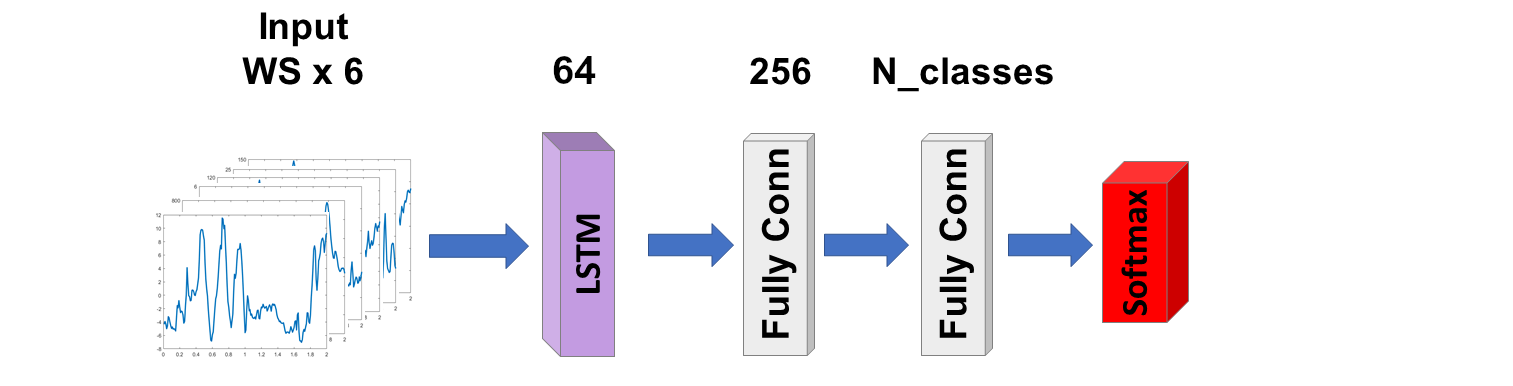
\includegraphics[width=\textwidth]{figure/lstm_model_64.png}
    \caption{Modello LSTM ridotto per il porting sullo smartwatch HEXIWEAR.}
    \label{fig:lstm-models-port}
\end{figure}
\chapter{Risultati}
\label{cap:risultati}

\section{Esperimenti su PC}
\label{sec:esperimenti-su-pc}

In questa sezione discutiamo i risultati degli esperimenti sui modelli proposti condotti in ambiente PC; innanzitutto analizziamo le migliori metriche ottenute dalla classificazione delle attività e degli utenti sia per il dataset costruito ad hoc che per il dataset DLA, in seguito studiamo le performance al variare della lunghezza della finestra di processing e delle feature calcolate ed infine mostriamo alcuni test di significatività parametrici.

\subsection{Metriche d'accuratezza}
\label{ssec:metriche-di-accuratezza}

Nella Tabella \ref{tab:activity-classification} possiamo vedere i risultati delle metriche ottenute dai quattro classificatori proposti sia sul dataset costruito ad hoc che sul dataset DLA; questi valori fanno riferimento ai migliori risultati ricavati da ogni modello durante un esperimento di 5-fold cross-validation variando la lunghezza della finestra di campionamento e, per i modelli classici, il numero di features; per ogni metrica è riportato in grassetto il miglior risultato fra i quattro modelli.

Nel caso del dataset ad hoc il classificatore SVM produce il miglior valore per la metrica di Recall (0.934), mentre LSTM ottiene la migliore Accuracy (0.947) e ERS-KNN produce le migliori Precision e F1-score(0.941 e 0.936); questo ci mostra come la classificazione dei lavaggi e delle sanificazioni attraverso segnali raccolti da smartwatch comuni sia un processo fattibile sia con gli strumenti standard di machine learning che con quelli più avanzati di deep learning. L'attività di sanificazione è quella con i risultati più bassi, circa l'82\%, ottenuta da CNN; questo è probabilmente dato dal fatto che le sanificazioni sono attività meno dinamiche rispetto ai lavaggi, dove l'uso dell'acqua induce vibrazioni più semplici da rilevare.

Per quanto riguarda il dataset DLA il modello CNN supera gli altri modelli in ogni metrica calcolata, nonostante questo le performance di ERS-KNN rimangono sopra al 91\%. Paragonato agli esperimenti sul dataset ad hoc le performance hanno subito una decrescita media dal 1\% fino all'8\% a seconda del classificatore. Questa riduzione di performance può essere causata dal numero maggiore di etichette; infatti nel dataset DLA abbiamo 10 etichette totali (scrittura, lavaggio mani, lavaggio volto, lavaggio denti, spazzare, passare l'aspirapolvere, mangiare, spolverare, strofinare, altro) le quali tendono a disperdere maggiormente i risultati. Un'altra causa può essere la mancanza di segnali del giroscopio che impattano significativamente sulle capacità di classificazione, in particolare dei modelli di machine learning classici.

\begin{table}
    \centering
    \begin{tabular}{l | c c | c c | c c | c c }
        \hline
        & \multicolumn{2}{c}{SVM} & \multicolumn{2}{c}{ERS-KNN} & \multicolumn{2}{c}{CNN} & \multicolumn{2}{c}{LSTM} \\
        \hline 
        & ad hoc & DLA & ad hoc & DLA & ad hoc & DLA & ad hoc & DLA \\
        Accuracy & 0.942 & 0.891 & 0.946 & 0.914 & 0.909 & \textbf{0.923} & \textbf{0.947} & 0.866 \\
        Precision & 0.936 & 0.907 & \textbf{0.941} & 0.931 & 0.898 & \textbf{0.939} & 0.911 & 0.882 \\
        Recall & \textbf{0.934} & 0.867 & 0.932 & 0.914 & 0.917 & \textbf{0.925} & 0.908 & 0.874 \\
        F1-score& 0.935 & 0.886 & \textbf{0.936} & 0.922 & 0.908 & \textbf{0.932} & 0.910 & 0.878\\
        \hline
    \end{tabular}
    \caption{Migliori risultati della classificazione delle attività ottenuti sia dal dataset costruito ad hoc che dal dataset DLA.}
    \label{tab:activity-classification}
\end{table}

\`E importante notare che per entrambi i dataset i risultati migliori sono stati ottenuti con finestre di lunghezza: SVM=12s, ERS-KNN=8s, CNN=6s, LSTM=2s e, nel caso di SVM ed ERS-KNN, utilizzando tutte le feature.

\subsection{Riconoscimento degli utenti}
\label{ssec:riconoscimento-degli-utenti}

Il secondo insieme di esperimenti ha lo scopo di identificare la persona che lava o sanifica le mani al posto dell'attività di per sé, per questo motivo abbiamo rimosso dai dataset tutti i sample che non fanno parte di queste categorie e abbiamo cambiato le etichette per identificare la persona piuttosto che l'attività. Nella Tabella \ref{tab:person-classification} possiamo vedere le migliori metriche ottenute dai quattro classificatori su entrambi i dataset. 

Il riconoscimento degli utenti è un compito più semplice rispetto al riconoscimento delle attività; per il dataset costruito ad hoc la migliore accuratezza è dello 0.99 ottenuta con il classificatore SVM, questo indica che le attività di lavaggio e sanificazione non strutturate contengono una sorta di impronta digitale che permette la facile identificazione dell'utente che le svolge. Inoltre da questo esperimento vediamo come le tecniche di machine learning classiche superano di cinque punti percentuali quelle di deep learning. Come nel caso del dataset costruito ad hoc, anche le metriche ricavate dal dataset DLA mostrano una maggiore semplicità nel riconoscere gli utenti rispetto l'attività; in questo caso i classificatori classici superano quelli di deep learning, ma, anche se gli esperimenti hanno una buona accuratezza (sopra il 95\%), in generale si ha comunque una riduzione nelle performance rispetto al dataset costruito ad hoc.

\begin{table}
    \centering
    \begin{tabular}{l | c c | c c | c c | c c}
        \hline
        & \multicolumn{2}{c}{SVM} & \multicolumn{2}{c}{ERS-KNN} & \multicolumn{2}{c}{CNN} & \multicolumn{2}{c}{LSTM} \\
        \hline
        & ad hoc & DLA & ad hoc & DLA & ad hoc & DLA & ad hoc & DLA \\
        \hline
        Accuracy  & \textbf{0.991} & 0.946 & 0.988 & \textbf{0.959} & 0.958 & 0.941 & 0.966 & 0.902 \\
        Precision & \textbf{0.990} & 0.949 & 0.985 & \textbf{0.957} & 0.945 & 0.940 & 0.959 & 0.902 \\
        Recall    & \textbf{0.989} & 0.942 & 0.986 & \textbf{0.949} & 0.952 & 0.943 & 0.956 & 0.903 \\
        F1-score  & \textbf{0.990} & 0.946 & 0.985 & \textbf{0.959} & 0.948 & 0.939 & 0.957 & 0.903 \\
        \hline
    \end{tabular}
    \caption{Migliori risultati della classificazione degli utenti ottenuti sia dal dataset costruito ad hoc che dal dataset DLA.}
    \label{tab:person-classification}
\end{table}

\subsection{Utilizzo di memoria e tempistiche}
\label{ssec:utilizzo-di-memoria-e-tempistiche}

Per valutare la complessità dei modelli di machine learning proposti, durante ogni esperimento, abbiamo misurato le performance e l'utilizzo di memoria di ogni classificatore; in particolare, i modelli sono stati implementati nella piattaforma Matlab2021a\textsuperscript{\textregistered} utilizzando gli strumenti di machine learning integrati e sono stati eseguiti su un PC desktop con una CPU Intel\textsuperscript{\textregistered} Core i9 equipaggiata con 32GB di memoria RAM ed una GPU Nvidia\textsuperscript{\textregistered} Quadro\textsuperscript{\textregistered} RTXTM 4000. Sia la fase di addestramento che quella d'inferenza sono state svolte impostando la GPU come ambiente d'esecuzione in modo da sfruttare a pieno le potenzialità del parallelismo CUDA\textsuperscript{\textregistered}.

La Tabella \ref{tab:memory} mostra le performance e l'utilizzo di memoria di ogni modello, come atteso la fase di addestramento dei modelli di deep learning è la più lunga con un massimo di 470 secondi misurati per l'LSTM, mentre l'ERS-KNN risulta essere il più veloce da addestrare con 5.8 secondi. Dal punto di vista dell'inferenza l'SVM sorpassa di molto gli altri modelli con 160$\mu$s; è importante notare che nel caso dell'SVM e dell'ERS-KNN le tempistiche prevedono anche l'estrazione delle feature il cui costo non è trascurabile nel momento del passaggio all'esecuzione sul dispositivo embedded.

\begin{table}
    \centering
    \begin{tabular}{l c c c c}
        \hline
        & SVM & ERS-KNN & CNN & LSTM \\
        \hline
        Tempo d'addestramento(s) & 7.191 & \textbf{5.803} & 299.551  & 472.069 \\
        Tempo d'inferenza(ms) & \textbf{0.016} & 0.331 & 0.505  & 1.749 \\
        Memoria utilizzata(MB) & \textbf{4.168} & 41.996& 6.389 & 5.569 \\
        \hline
    \end{tabular}
    \caption{Tempo d'addestramento, tempo d'inferenza e memoria utilizzata dai modelli eseguiti in ambiente PC.}
    \label{tab:memory}
\end{table}

\subsection{Lunghezza della finestra}
\label{ssec:lunghezza-della-finestra}

La dimensione della finestra di processing influisce in molti modi sulla classificazione dei modelli; di seguito analizziamo nel dettaglio i risultati degli esperimenti su questa dipendenza. Sia SVM che ERS-KNN (Figura \ref{fig:window:svm} e Figura \ref{fig:window:knn}) mostrano un trend delle performance pressoché piano, anche se da un certo punto in poi le metriche iniziano a deteriorarsi; in particolare l'SVM vede un miglioramento delle performance fino ad una finestra di dimensione 12 secondi dopodiché Precision, Recall ed F1-score diminuiscono. In maniera del tutto simile, le performance dell'ERS-KNN aumentano fino ad una finestra di 8 secondi. Un trend opposto si può vedere nei risultati ottenuti dai classificatori deep learning (Figura \ref{fig:window:cnn} e Figura \ref{fig:window:lstm}), in questo caso le metriche mostrano un decremento monotono all'aumentare della finestra.

\begin{figure}[!htb]
    \centering
    \begin{subfigure}{.45\textwidth}
        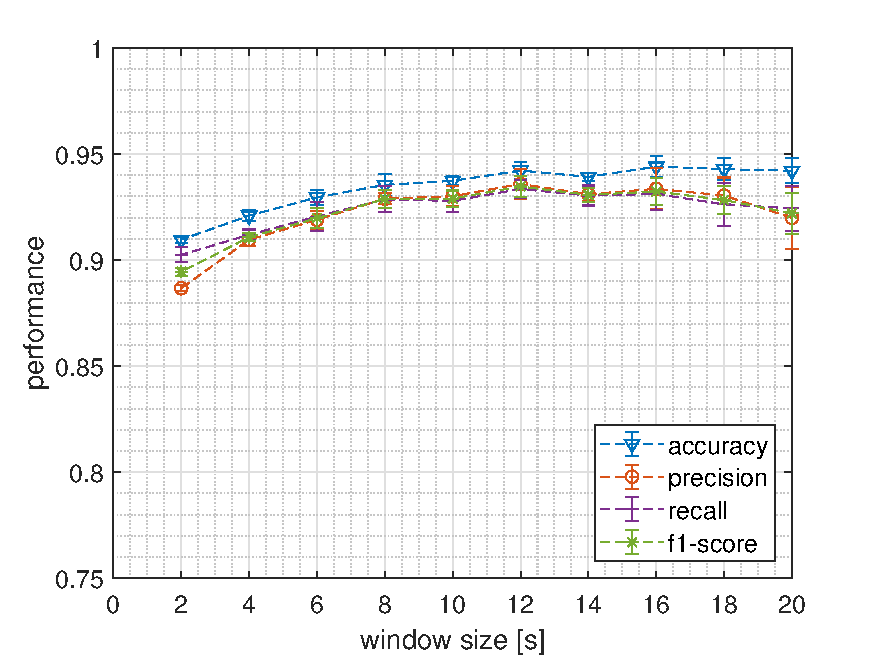
\includegraphics[width=\textwidth]{figure/svm_window.pdf}
        \caption{SVM}
        \label{fig:window:svm}
    \end{subfigure}
    \begin{subfigure}{.45\textwidth}
        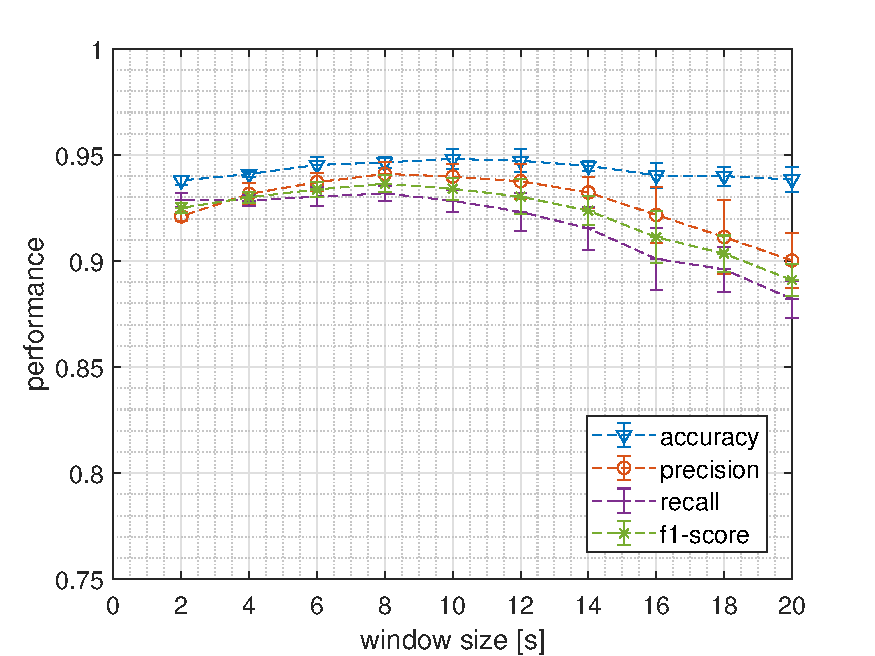
\includegraphics[width=\textwidth]{figure/knn_window.pdf}
        \caption{ERS-KNN}
        \label{fig:window:knn}
    \end{subfigure}
    \begin{subfigure}{.45\textwidth}
        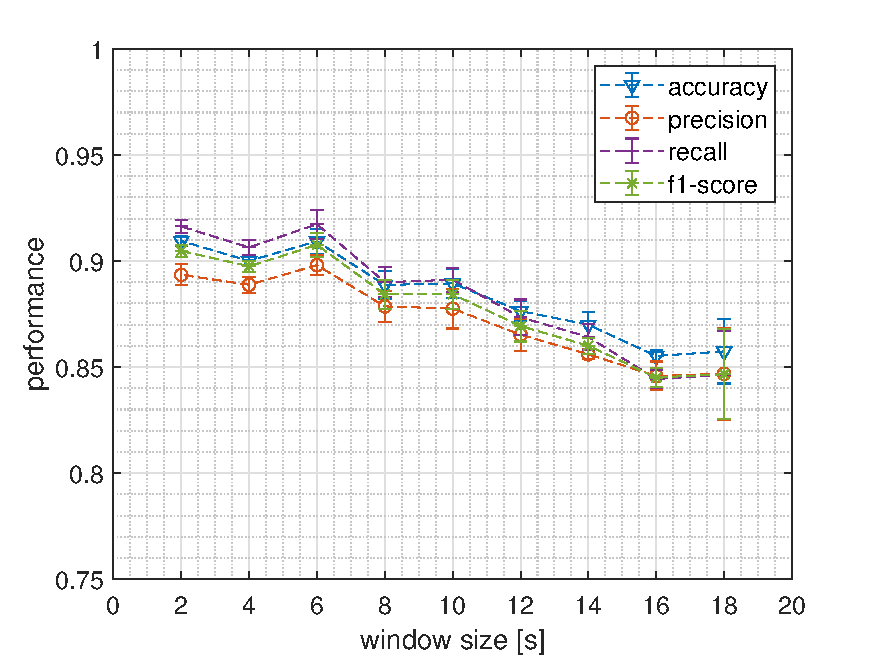
\includegraphics[width=\textwidth]{figure/cnn_window.pdf}
        \caption{CNN}
        \label{fig:window:cnn}
    \end{subfigure}
    \begin{subfigure}{.45\textwidth}
        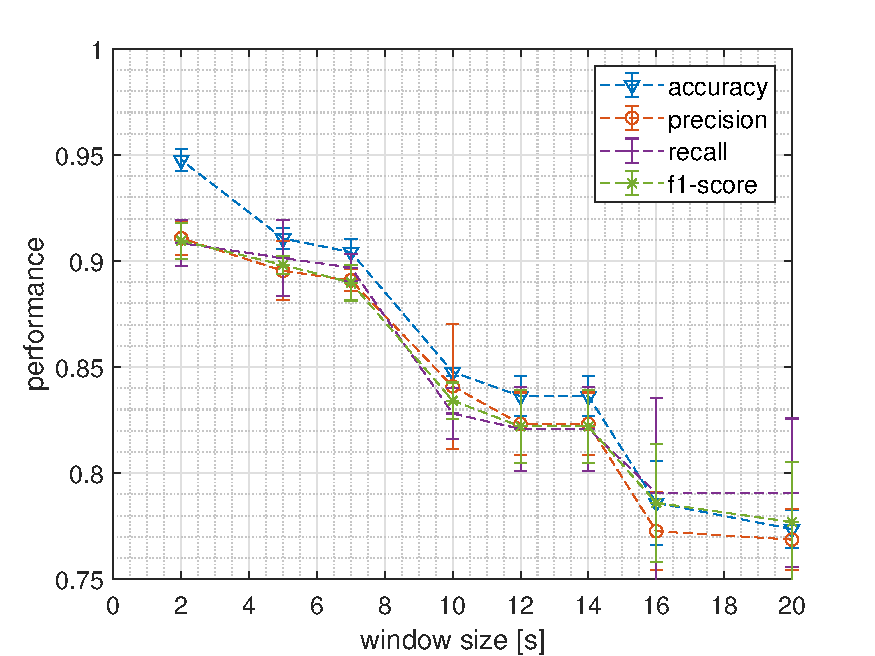
\includegraphics[width=\textwidth]{figure/lstm_window.pdf}
        \caption{LSTM}
        \label{fig:window:lstm}
    \end{subfigure}
    \caption{Performance dei modelli SVM(a), ERS-KNN(b), CNN(c) ed LSTM(d) al variare della lunghezza della finestra di processing.}
    \label{fig:window}
\end{figure}

\subsection{Selezione delle feature}
\label{ssec:selezione-delle-feature}

Oltre alla lunghezza della finestra di processing un altro parametro che influisce sulle prestazioni dei modelli di machine learning classici sono le feature che vengono calcolate. Per selezionare le feature utilizziamo un metodo detto di \textit{forward feature selection} il quale sfrutta l'accuratezza come criterio per valutare l'impatto dell'aggiunta di nuove feature partendo da un insieme vuoto fino all'esaurimento. Ogni gruppo di feature Base(B), Hjorth(H) e Shape(S) è trattato come una sola unità che può essere aggiunta o rimossa. Innanzitutto abbiamo testato i classificatori con un singolo gruppo di feature per poi aggiungere gli altri gruppi esplorando tutte le combinazioni.

La Tabella \ref{tab:features} mostra le performance per entrambi i classificatori al variare dei gruppi di feature selezionati. Le metriche mostrano tutte un aumento monotono che raggiunge le performance migliori nel momento in cui tutti i gruppi sono usati assieme; questo significa che ogni gruppo di feature aggiunge informazioni utili al processo di classificazione, inoltre, il gruppo Hjorth è quello che contiene le informazioni più utili essendo quello con  i risultati migliori dei tre gruppi quando testati da soli. 

Dal punto di vista implementativo possiamo fare un compromesso tra prestazioni e complessità computazionale scegliendo di calcolare solo le feature Base + Hjorth rinunciando allo 0.2\% delle prestazioni o, addirittura, calcolando solo le Hjorth ottenendo una precisione del 92\%, ma risparmiando molte risorse computazionali.

\begin{table}
    \centering
    \begin{tabular}{l l c c c c c c c}
        \hline
        & & B     & H     & S     & B+H   & B+S   & H+S   & B+H+S \\
        \hline
        \multirow{2}{*}{Accuracy}   & SVM & 0.901 & 0.923 & 0.339 & 0.941 & 0.916 & 0.926 & \textbf{0.942} \\
                                    & KNN & 0.904 & 0.908 & 0.719 & 0.944 & 0.908 & 0.922 & \textbf{0.946} \\
        \hline
        \multirow{2}{*}{Precision}  & SVM & 0.892 & 0.912 & 0.500 & 0.932 & 0.910 & 0.917 & \textbf{0.936} \\      
                                    & KNN & 0.899 & 0.908 & 0.683 & 0.937 & 0.909 & 0.920 & \textbf{0.941} \\
        \hline
        \multirow{2}{*}{Recall}     & SVM & 0.891 & 0.913 & 0.480 & 0.932 & 0.906 & 0.921 & \textbf{0.934} \\
                                    & KNN & 0.873 & 0.889 & 0.674 & 0.929 & 0.886 & 0.902 & \textbf{0.932} \\
        \hline
        \multirow{2}{*}{F1-score}   & SVM & 0.891 & 0.891 & 0.490 & 0.932 & 0.908 & 0.919 & \textbf{0.935} \\
                                    & KNN & 0.886 & 0.886 & 0.678 & 0.933 & 0.897 & 0.911 & \textbf{0.936} \\
        \hline
    \end{tabular}
    \caption{Risultato della selezione delle feature applicata ai due modelli di machine learning classici.}
    \label{tab:features}
\end{table}

\subsection{Test di significatività non parametrici}
\label{ssec:tesi-di-significativita-non-parametrici}

Dopo aver svolto tutti gli esperimenti sui modelli di machine learning visti in precedenza ed aver analizzato i loro risultati cerchiamo un metodo in grado di comparare questi modelli con la precisione statistica. Per questo utilizziamo tre variazioni del test di McNemar\cite{fagerland2013mcnemar}:

\begin{enumerate}
    \item test asintotico
    \item test del p-value medio
    \item test condizionale esatto
\end{enumerate}

Questo tipo di test è spesso usato in medicina per valutare gli effetti dei trattamenti, e, negli ultimi anni, nell'ambito del machine learning per comparare due modelli di grandi dimensioni senza doverli addestrare più volte. Il test di McNemar si assicura che il disaccordo fra i due casi corrisponda, commentando sul fatto che i due modelli siano in disaccordo fra loro (oppure non lo siano affatto); questo test non dice nulla sul fatto che uno dei due modelli sia più o meno accurato dell'altro.

La Tabella \ref{tab:mc-nemar-results} mostra i risultati dei tre test condotti per ogni coppia di classificatori.
Per ogni test, viene riportato il valore booleano $h$ che rappresenta la decisione del test quando si verifica l'ipotesi nulla, ovvero che i due classificatori abbiamo la stessa accuratezza nella predizione del risultato atteso.
Inoltre, viene riportato anche il valore $p$ che indica quanto è forte l'evidenza nel rifiutare o meno l'ipotesi nulla; ad esempio, quando si confrontano ERS-KNN con SVM, le tre varianti del test di McNemar concordano sull'accettare l'ipotesi nulla mentre, sia per ERS-KNN/LSTM che ERS-KNN/CNN, l'ipotesi nulla deve essere rifiutata. In questi casi, il valore $p$ per ogni test è vicino allo zero, rivelando una forte prova nel rifiutare l'ipotesi nulla.

Anche il confronto tra SVM/LSTM, SVM/CNN, e LSTM/CNN, porta a forti rifiuti dell'ipotesi nulla con p-value molto vicini allo zero, infatti, in questo scenario, solo gli strumenti di machine learning standard, ovvero SVM e ERS-KNN, possono essere considerati statisticamente equivalenti dal punto di vista delle prestazioni di classificazione.

\begin{table}
    \centering
    \begin{tabular}{c | l | c c | c c | c c }
        \hline
        & & \multicolumn{2}{c}{SVM} & \multicolumn{2}{c}{LSTM} & \multicolumn{2}{c}{CNN} \\
        \hline
                                &            & h     & p    & h    & p                      & h    & p \\
        \hline
        \multirow{3}{*}{KNN}    & asint.     & falso & $0.65$ & vero & $4.14 \times 10^{-25}$ & vero & $2.04 \times 10^{-21}$ \\
                                & p medio    & falso & $0.65$ & vero & $1.33 \times 10^{-25}$ & vero & $3.12 \times 10^{-27}$ \\
                                & esatto     & falso & $0.69$ & vero & $1.82 \times 10^{-32}$ & vero & $1.12 \times 10^{-22}$ \\
        \hline
        \multirow{3}{*}{SVM}    & asint.     &       &        & vero & $3.94 \times 10^{-05}$ & vero & $4.53 \times 10^{-22}$ \\
                                & p medio    &       &        & vero & $3.87 \times 10^{-05}$ & vero & $1.27 \times 10^{-18}$ \\
                                & esatto     &       &        & vero & $4.46 \times 10^{-05}$ & vero & $3.43 \times 10^{-22}$ \\
        \hline
        \multirow{3}{*}{LSTM}   & asint.     &       &        &      &                        & vero & $1.23 \times 10^{-25}$ \\
                                & p medio    &       &        &      &                        & vero & $5.13 \times 10^{-25}$ \\
                                & esatto     &       &        &      &                        & vero & $2.26 \times 10^{-24}$ \\ 
        \hline
    \end{tabular}
    \caption{Risultati dei tre test di McNemar sui modelli proposti.}
    \label{tab:mc-nemar-results}
\end{table}

\section{Esperimenti sull'HEXIWEAR}
\label{sec:esperimenti-sull-hexiwear}

In questa sezione discutiamo i risultati degli esperimenti condotti sui modelli proposti all'interno del dispositivo indossabile HEXIWEAR; a differenza degli esperimenti condotti su PC in questo caso viene utilizzato solo il dataset costruito ad hoc. Inizialmente analizziamo l'esito delle metriche di classificazione delle attività per il modello SVM al variare della lunghezza della finestra di processing e del numero di feature calcolate, in seguito studiamo le performance del modello LSTM al variare dei parametri interni utilizzati ed infine osserviamo le migliori prestazioni ottenute dai modelli in termini di tempo d'esecuzione, di memoria utilizzata e di consumo di energia da parte del dispositivo.

\subsection{Lunghezza della finestra di SVM}
\label{ssec:lunghezza-della-finestra-hexi}

Di seguito esaminiamo la variazione delle performance del modello SVM al variare della lunghezza della finestra di processing; la Figura \ref{fig:metrics-svm-window-hexi} mostra un cambiamento generale delle performance molto ampio con dei picchi massimi per le finestre di lunghezza 12 secondi e 14 secondi e dei picchi minimi per finestre di lunghezza 8 secondi, 10 secondi e 20 secondi, in base alle metriche. In particolare, notiamo che tutti i risultati si comportano pressoché allo stesso modo al variare della lunghezza della finestra, anche se l'accuratezza supera gli altri di sei punti percentuali, questo è sinonimo di una buona correlazione fra i valori.

\begin{figure}[!htb]
    \centering
    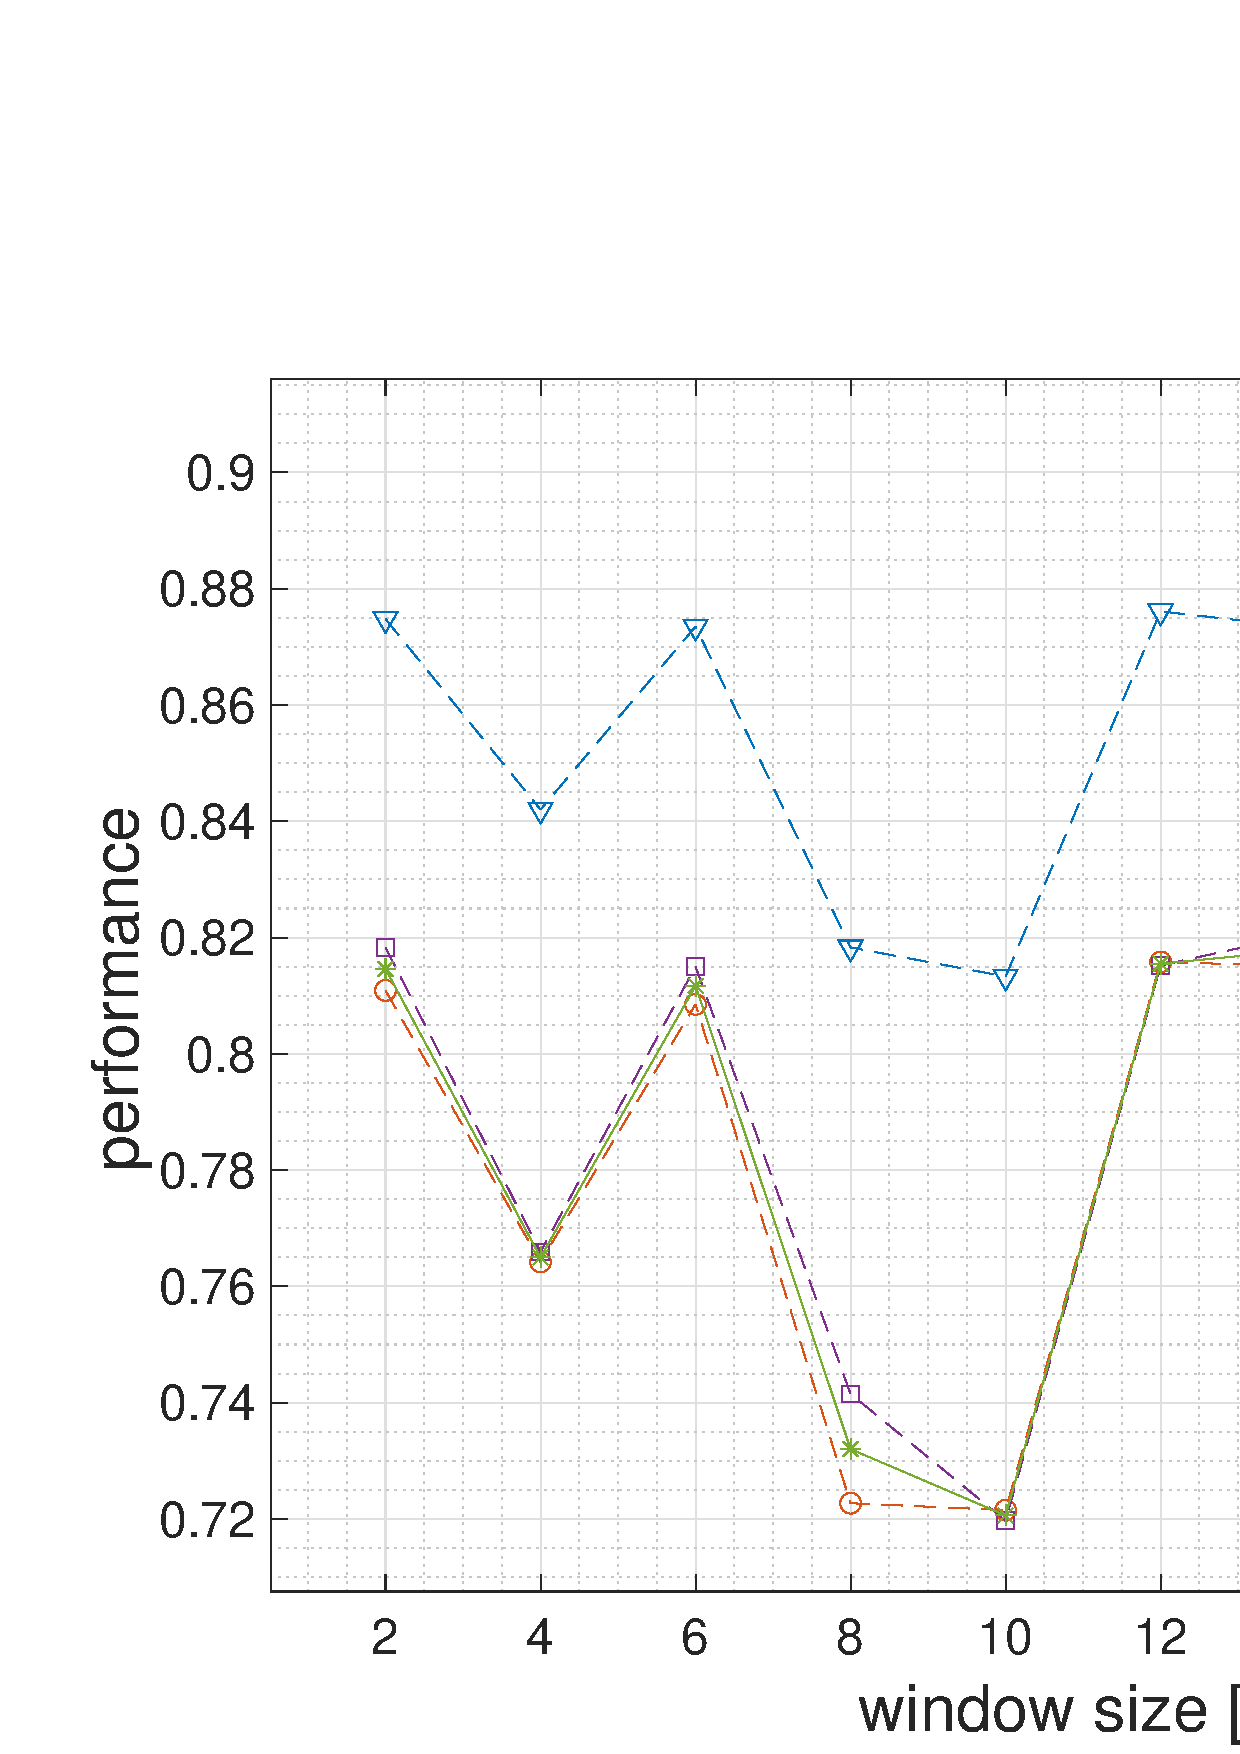
\includegraphics[width=.8\textwidth]{figure/svm_performance.pdf}
    \caption{Metriche ricavate dal modello SVM al variare della lunghezza della finestra.}
    \label{fig:metrics-svm-window-hexi}
\end{figure}

Paragonate alle performance calcolate su PC (Figura \ref{fig:window:svm}) nel caso del porting notiamo un generale peggioramento; inoltre osserviamo come su PC tutte le metriche mantengono un valore superiore al 90\% arrivando, nel caso dell'accuratezza, quasi al 95\%, mentre nel caso del porting le metriche non superano mai il 90\%, con il valore massimo dell'accuratezza al 88\%. Questo fenomeno non ci sorprende poiché è sicuramente causato dalla riduzione di capacità che abbiamo dovuto apportare ai modelli durante la fase di porting.

\subsection{Selezione delle feature di SVM}
\label{ssec:selezione-delle-feature-di-svm-hexi}

Il secondo esperimento condotto sul classificatore SVM consiste nel variare le feature calcolate ed osservare il cambiamento delle performance che ne segue. 
Come nel caso degli esperimenti condotti su PC (Sezione \ref{ssec:selezione-delle-feature}) utilizziamo il metodo di \textit{forward feature selection} per scegliere i gruppi di feature da valutare; nel porting sul dispositivo HEXIWEAR si è scelto di ridurre il numero di feature calcolate in modo da diminuire la memoria richiesta, di conseguenza le feature calcolate appartengono tutte al gruppo Base e sono: Media(A), Deviazione Standard(S), Massimo e Minimo(M).
Ogni esperimento è stato condotto utilizzando una finestra di processing di 12 secondi; per prima cosa abbiamo testato il classificatore con un singolo gruppo di feature per poi aggiungere progressivamente gli altri gruppi ed esplorare tutte le combinazioni.

La Tabella \ref{tab:metrics-svm-feat-hexi} mostra le performance al variare dei gruppi di feature calcolati; anche in questo caso le metriche presentano un aumento monotono raggiungendo le performance migliori quando tutti i gruppi sono usati assieme, poiché ogni feature aggiunge informazioni utili alla classificazione. A differenza delle altre metriche, la Recall ha un valore maggiore nel caso di \textit{Media + Deviazione Standard}; infatti questi due gruppi sono quelli che producono i risultati migliori se si esclude la combinazione di tutti tre. Inoltre il gruppo che contiene le informazioni più utili è quello della Media, producendo i risultati migliori quando preso singolarmente; mentre Deviazione Standard e Massimo e Minimo lo seguono di poco.

\begin{table}
    \centering
    \begin{tabular}{l c c c c c c c}
        \hline
        & A & S & M & A+S & A+M & S+M & A+S+M \\
        \hline
        Accuracy & 0.7946 & 0.7734 & 0.7770 & 0.8697 & 0.8589 & 0.7946 & \textbf{0.8761} \\
        Precision & 0.6638 & 0.6481 & 0.6402 & 0.7919 & 0.7818 & 0.6638 & \textbf{0.8158} \\
        Recall & 0.6682 & 0.6516 & 0.6701 & \textbf{0.8218} & 0.8021 & 0.6682 & 0.8152 \\
        F1-Score & 0.6660 & 0.6499 & 0.6548 & 0.8065 & 0.7918 & 0.6660 & \textbf{0.8155} \\
        \hline
    \end{tabular}
    \caption{Metriche ricavate dal modello SVM al variare delle feature calcolate.}
    \label{tab:metrics-svm-feat-hexi}
\end{table}

\subsection{Selezione dei parametri di LSTM}
\label{ssec:selezione-dei-parametri-di-lstm-hexi}

L'ultimo esperimento che prendiamo in esame sull'HEXIWEAR riguarda le performance del modello di deep learning LSTM variando alcuni dei suoi parametri interni. 
La rete LSTM caricata sull'HEXIWEAR (Figura \ref{fig:lstm-models-port}) è composta dal un singolo modulo LSTM e da due livelli densamente connessi; nel seguente esperimento abbiamo preso come parametri interni il numero di unità nel modulo LSTM ed il numero di neuroni nascosti all'interno del primo livello densamente connesso, mentre l'ultimo livello denso è stato settato costante pari al numero di etichette. 

In Tabella \ref{tab:metrics-lstm-param-hexi} vediamo le metriche calcolate al variare dei seguenti parametri: 64/256, 32/128, 16/64, 8/32, in cui il primo numero rappresenta il parametro del modulo LSTM ed il secondo rappresenta il numero di neuroni nello strato denso. 

Come possiamo immaginare il modello che produce i risultati migliori è quello con i parametri 64/256 con un'Accuracy dell'87\%, ed una Recall dell'88\% anche se gli altri modelli mostrano una riduzione lineare delle performance solo di circa il 3\% ad ogni riduzione dei parametri della rete.

\begin{table}
    \centering
    \begin{tabular}{l c c c c}
        \hline
        & \multicolumn{4}{c}{Parametri interni} \\
        \hline
        & 64/256 & 32/128 & 16/64 & 8/32 \\
        \hline
        Accuracy & \textbf{0.877} & 0.849 & 0.812 & 0.774 \\
        Precision & \textbf{0.879} & 0.849 & 0.809 & 0.764 \\
        Recall & \textbf{0.880} & 0.854 & 0.799 & 0.759 \\
        F1-score & \textbf{0.880} & 0.852 & 0.804 & 0.761 \\
        \hline
    \end{tabular}
    \caption{Metriche ricavate dal modello LSTM al variare dei parametri interni.}
    \label{tab:metrics-lstm-param-hexi}
\end{table}

\subsection{Utilizzo di memoria e tempistiche}
\label{ssec:utilizzo-di-memoria-e-tempistiche-hexi}

Per valutare meglio le performance complessive dei modelli di machine learning eseguiti sullo smartwatch HEXIWEAR, durante ogni esperimento abbiamo misurato le tempistiche, il consumo di memoria e l'energia di ogni classificatore.

La Tabella \ref{tab:memory-hexi} mostra i modelli con i risultati migliori fra quelli visti negli esperimenti precedenti. I parametri tempo e memoria dei sensori rappresentano il tempo in millisecondi e la memoria in byte occupati durante la fase di raccolta dei dati non elaborati dai sensori di accelerometro e giroscopio; questi due valori dipendono fortemente dalla lunghezza della finestra di processing, per questo motivo sono uguali per i due modelli SVM, che utilizzano entrambi una finestra di 12 secondi, e sono minori per il modello LSTM, che invece fa uso di una finestra di 2 secondi.

Il tempo e la memoria occupata per il calcolo delle feature sono presenti solo nei modelli SVM e, come possiamo immaginare, sono minori nel caso in cui viene calcolato un numero minore di feature. Per quanto riguarda il tempo d'inferenza notiamo una piccola differenza fra i modelli SVM, mentre il modello LSTM impiega circa il doppio del tempo, invece la memoria impiegata per l'inferenza ha valori simili fra LSTM e l'esperimento SVM con la finestra ed è minore per l'SVM con meno feature. Infine vediamo che la potenza è maggiore per il modello LSTM ed è simile fra i due modelli SVM, con l'esperimento sulle feature che ha la potenza minore.

\begin{table}
    \centering
    \begin{tabular}{l c c c}
        \hline
        & SVM window & SVM feature & LSTM \\
        \hline
        t. sensori [ms] & 10798 & 10798 & \textbf{1800} \\
        t. feature [$\mu$s] & 1161 & \textbf{226} & - \\
        t. inferenza [ms] & 52 & \textbf{48} & 85 \\
        \hline
        mem. sensori [B] & 28975 & 28975 & \textbf{4975} \\
        mem. feature [B] & 29016 & \textbf{28944} & - \\
        mem. inferenza [B] & 10398 & \textbf{4390} & 13401 \\
        mem. modello [B] & 126989 & \textbf{68625} & 111040 \\
        \hline
        potenza [mW] & 8.47 & \textbf{8.42} & 13.03 \\
        \hline
    \end{tabular}
    \caption{Tempistiche d'esecuzione, memoria utilizzata e consumo d'energia dei modelli eseguiti sul dispositivo HEXIWEAR.}
    \label{tab:memory-hexi}
\end{table}

L'ultima analisi svolta consiste nel paragonare alcune delle metriche di tempo, memoria ed energia con il valore della loss per i modelli presi in esame; la funzione loss indica il costo in termini di prestazioni del modello ed è pari ad $1 - Accuracy$.

I grafici in Figura \ref{fig:performance-svm-hexi} riportano sull'\textit{asse x} il valore della loss e sull'\textit{asse y} la memoria totale ed il consumo di energia paragonando il modello SVM dell'esperimento sulla lunghezza della finestra di processing con quello sul calcolo delle feature. 
Nei grafici memoria totale vs. loss (Figura \ref{fig:performance-svm-hexi:svm-memory-loss-window} e Figura \ref{fig:performance-svm-hexi:svm-memory-loss-feature}) vediamo che i classificatori migliori risultano essere quello con una finestra di lunghezza 2 e quello con le feature calcolate A+M, poiché sono i due ad avere un basso utilizzo di memoria mantenendo anche un valore per la loss basso; allo stesso modo nei grafici consumo d'energia vs. loss (Figura \ref{fig:performance-svm-hexi:svm-power-loss-window} e Figura \ref{fig:performance-svm-hexi:svm-power-loss-feature}) i migliori risultano essere quello con finestra di lunghezza 12 e quello con le feature calcolate A+S.

Analogamente i grafici in Figura \ref{fig:performance-lstm-hexi} confrontano il valore della loss con l'energia, il tempo d'inferenza ed il peso del modello LSTM nell'esperimento sulla variazione dei parametri interni. Come vediamo tutti e tre i grafici mostrano una repentina diminuzione dei valori all'aumentare della loss, ovvero quando vengono considerati modelli con un numero minore di parametri interni. In tutti e tre i casi il classificatore con le migliori performance rispetto alla loss risulta essere quello con 32 unità LSTM e 128 neuroni nel primo strato nascosto.

\begin{figure}[!htbp]
    \centering
    \begin{subfigure}[t]{.45\textwidth}
        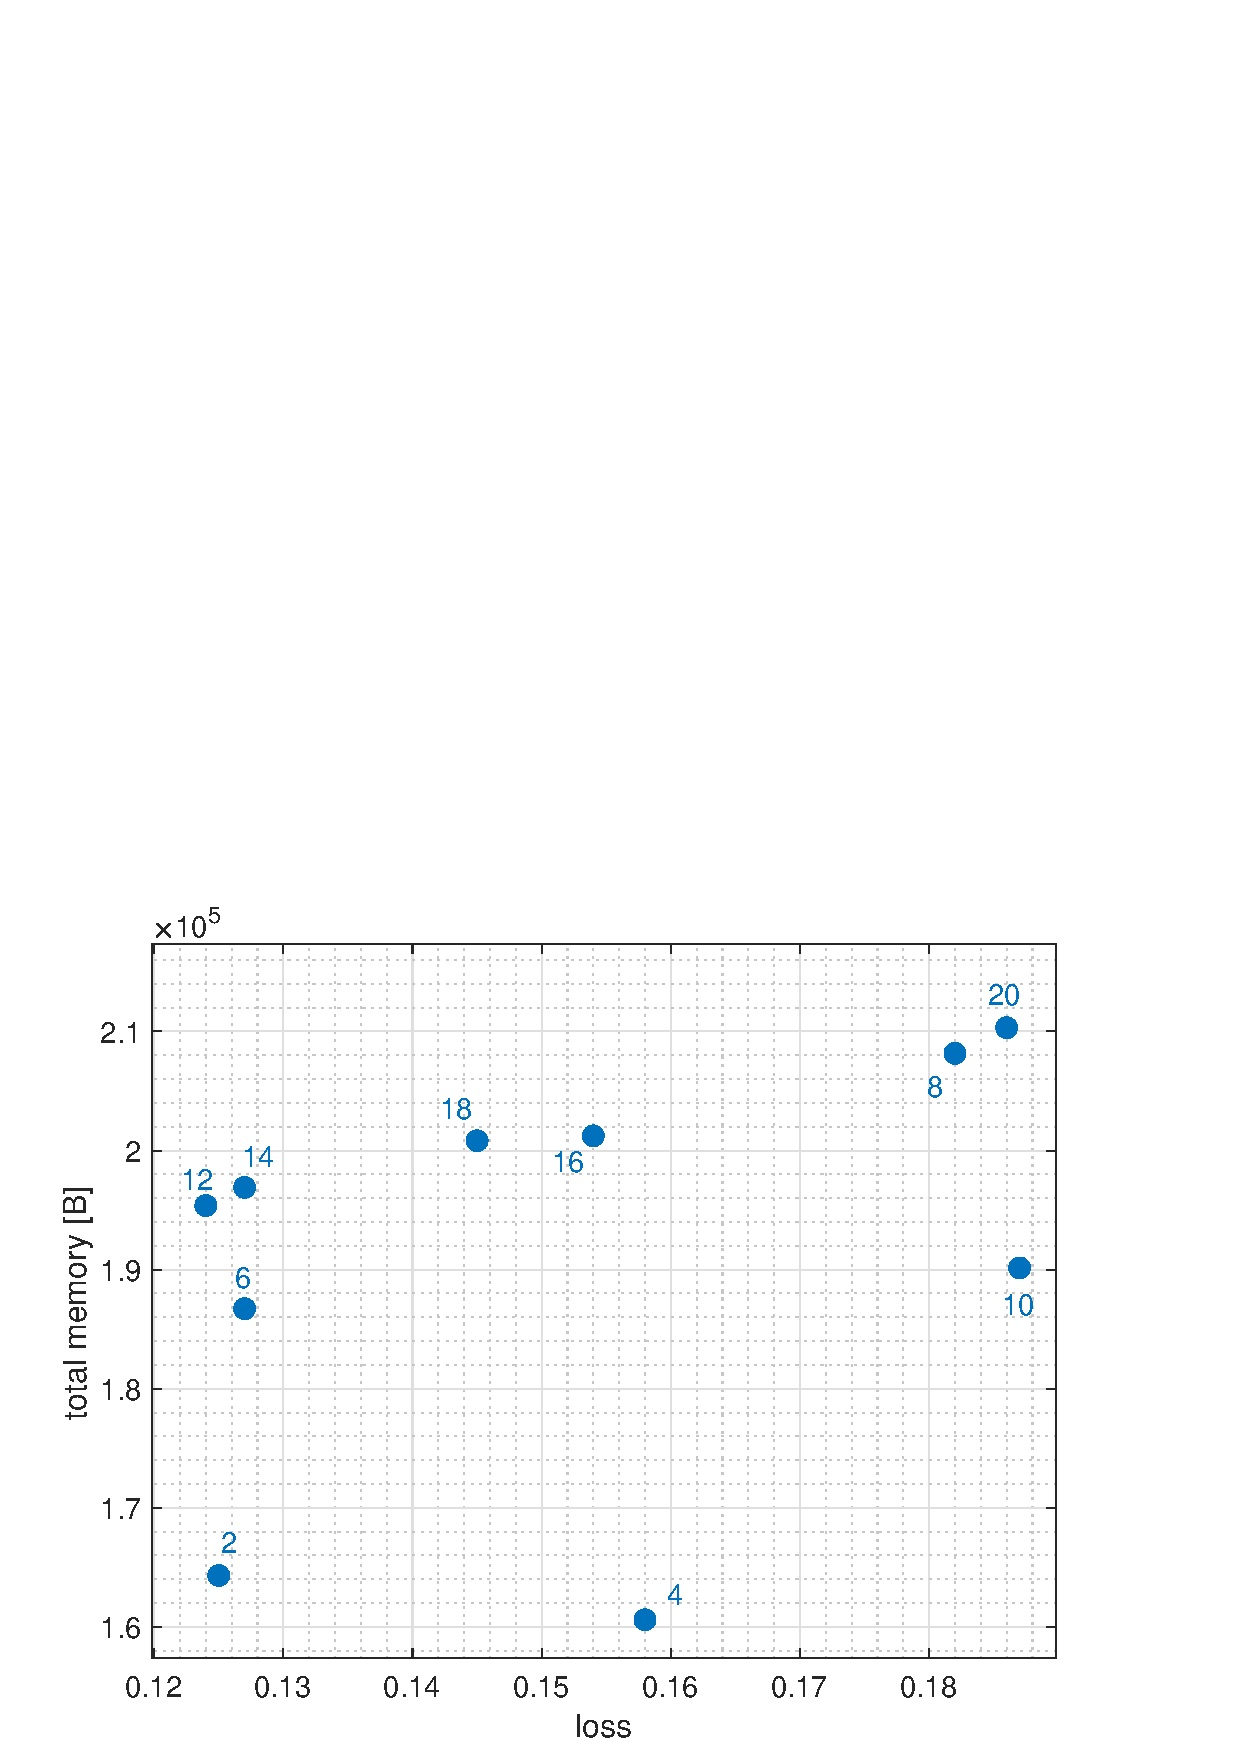
\includegraphics[width=\textwidth]{figure/svm_window_loss_memory.pdf}
        \caption{memoria totale vs. loss per gli esperimenti sulla lunghezza della finestra}
        \label{fig:performance-svm-hexi:svm-memory-loss-window}
    \end{subfigure}
    \begin{subfigure}[t]{.45\textwidth}
        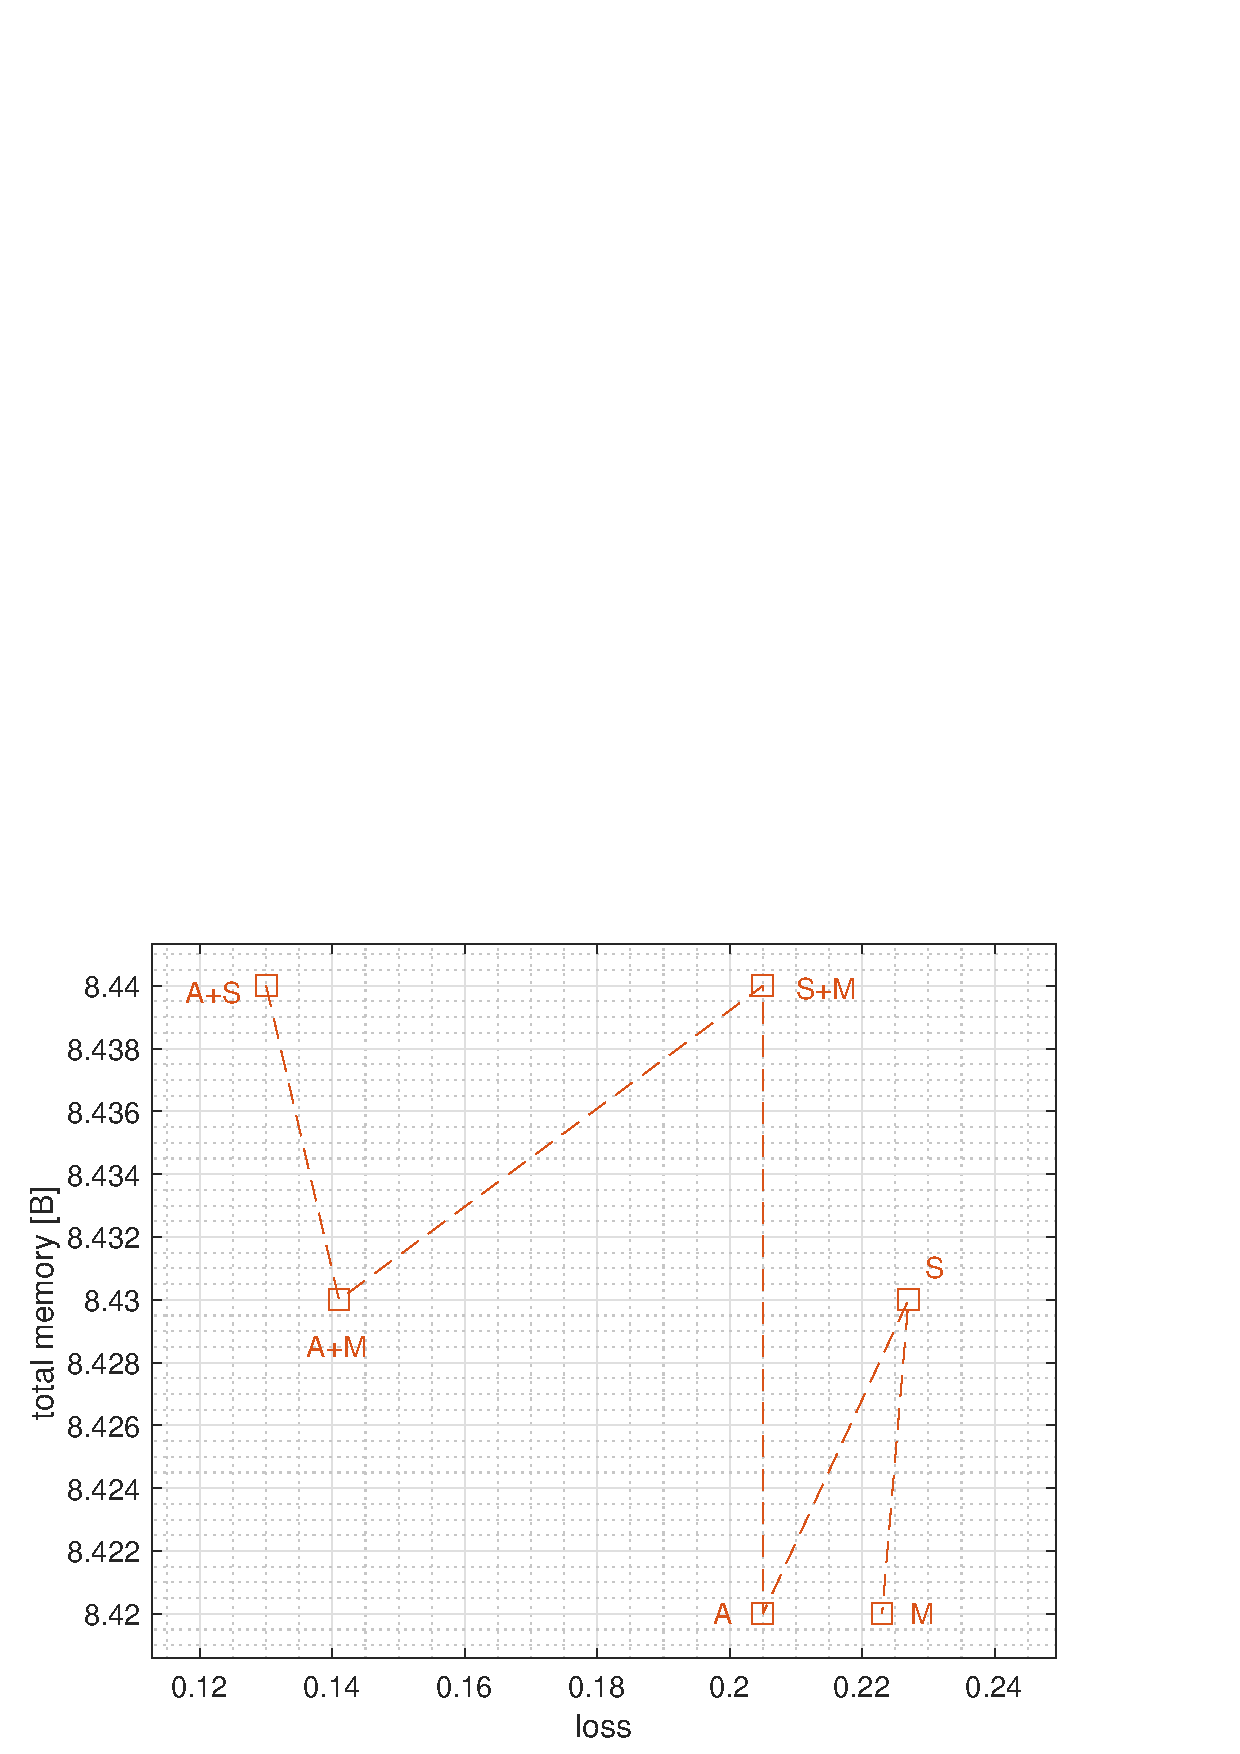
\includegraphics[width=\textwidth]{figure/svm_feat_loss_memory.pdf}
        \caption{memoria totale vs. loss per gli esperimenti sulle feature calcolate}
        \label{fig:performance-svm-hexi:svm-memory-loss-feature}
    \end{subfigure}
    \begin{subfigure}[t]{.45\textwidth}
        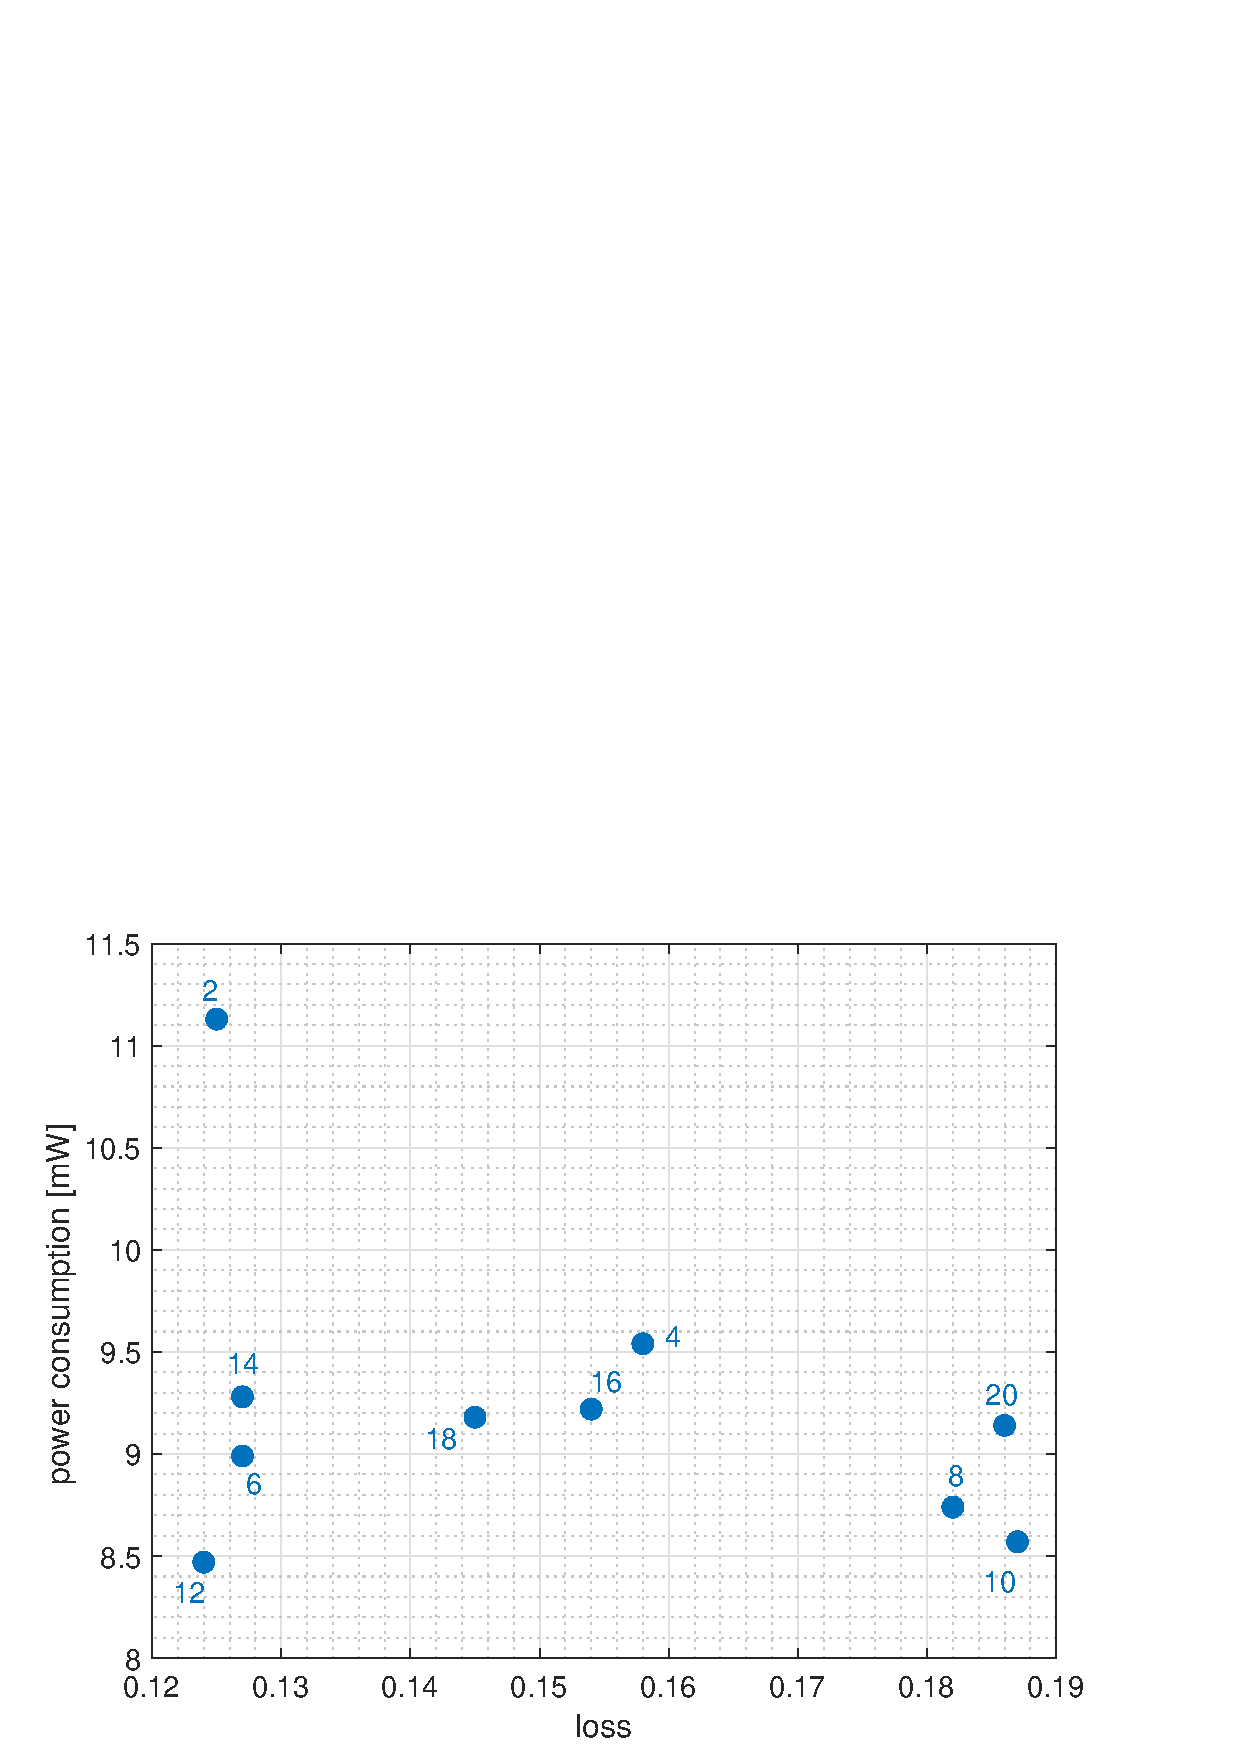
\includegraphics[width=\textwidth]{figure/svm_window_loss_power.pdf}
        \caption{consumo d'energia vs. loss per gli esperimenti sulla lunghezza della finestra}
        \label{fig:performance-svm-hexi:svm-power-loss-window}
    \end{subfigure}
    \begin{subfigure}[t]{.45\textwidth}
        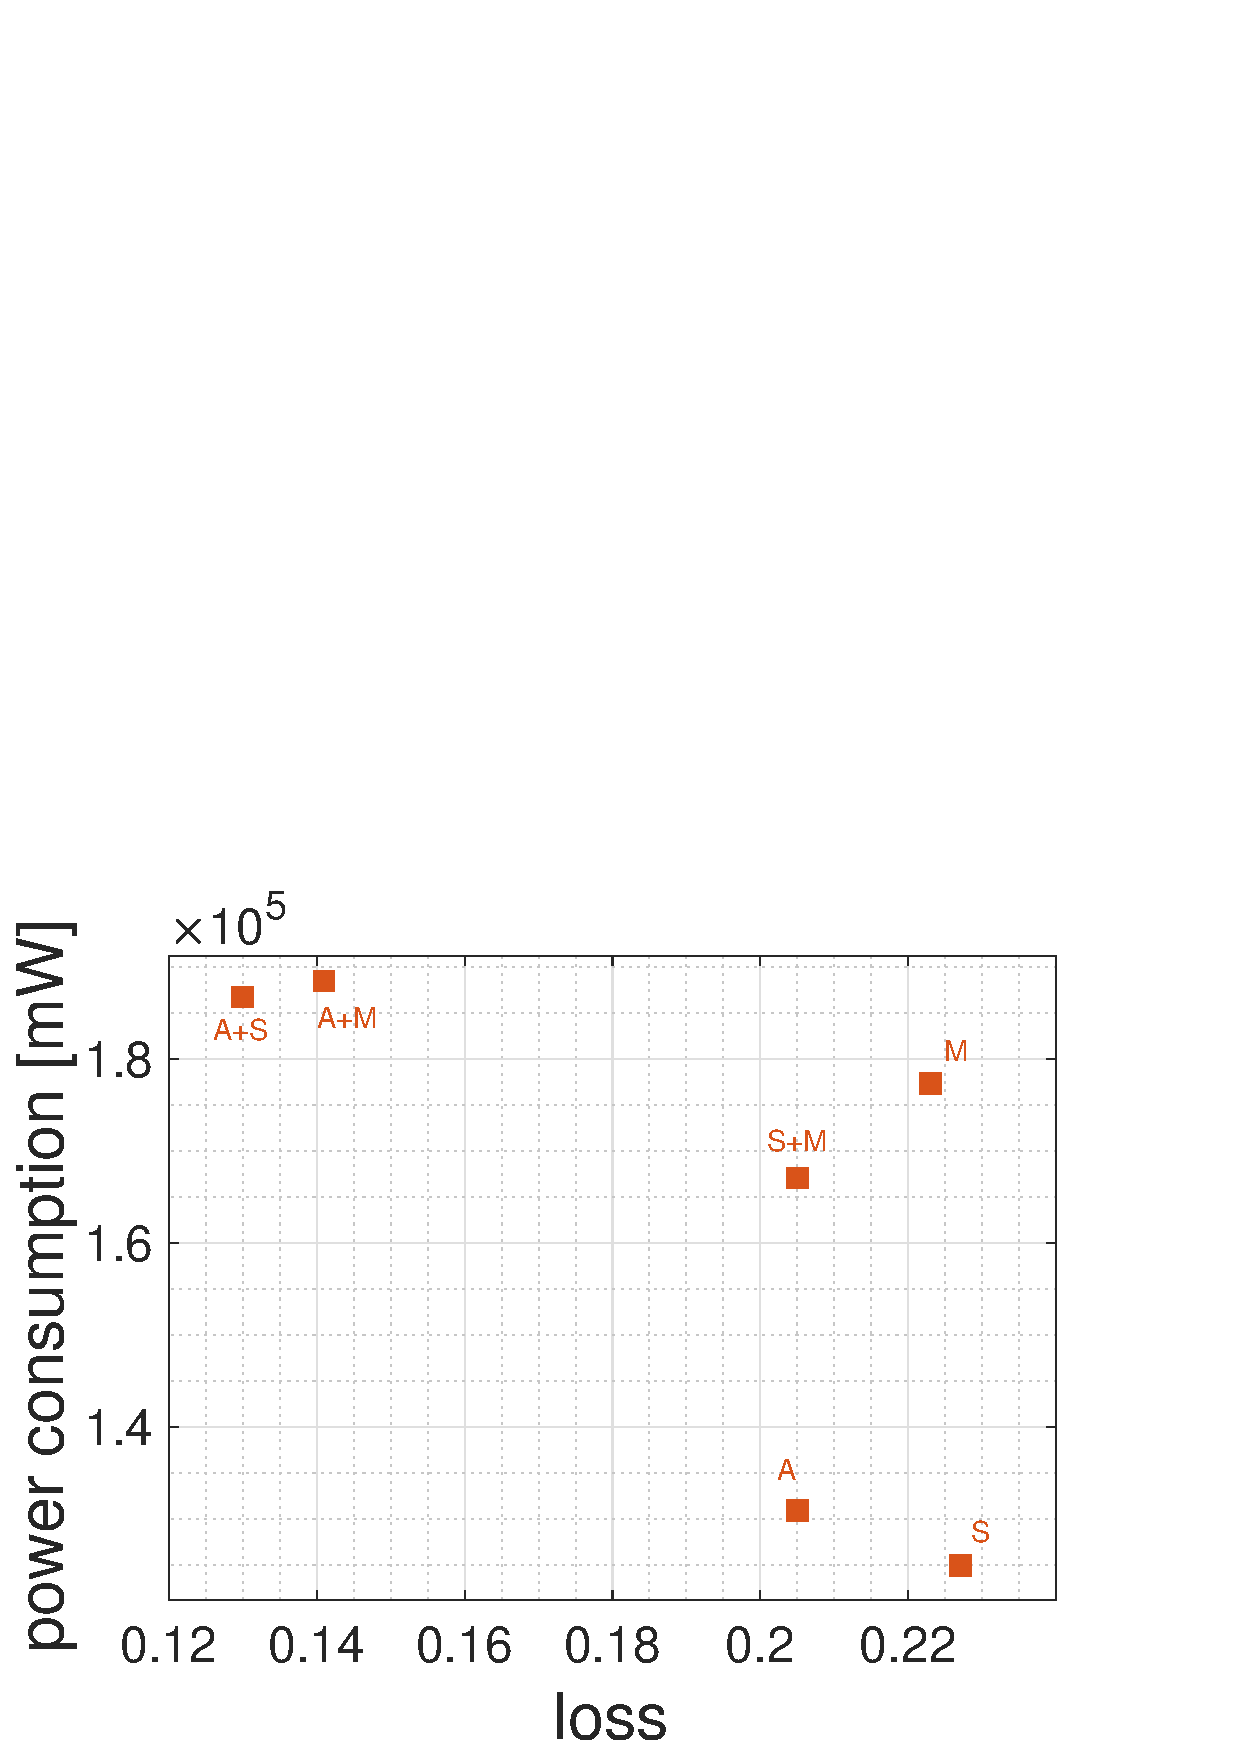
\includegraphics[width=\textwidth]{figure/svm_feat_loss_power.pdf}
        \caption{consumo d'energia vs. loss per gli esperimenti sulle feature calcolate}
        \label{fig:performance-svm-hexi:svm-power-loss-feature}
    \end{subfigure}
    \caption{Grafici prodotti dai modelli SVM confrontando memoria totale e consumo d'energia con la loss.}
    \label{fig:performance-svm-hexi}
\end{figure}

\begin{figure}[!htb]
    \centering
    \begin{subfigure}{.45\textwidth}
        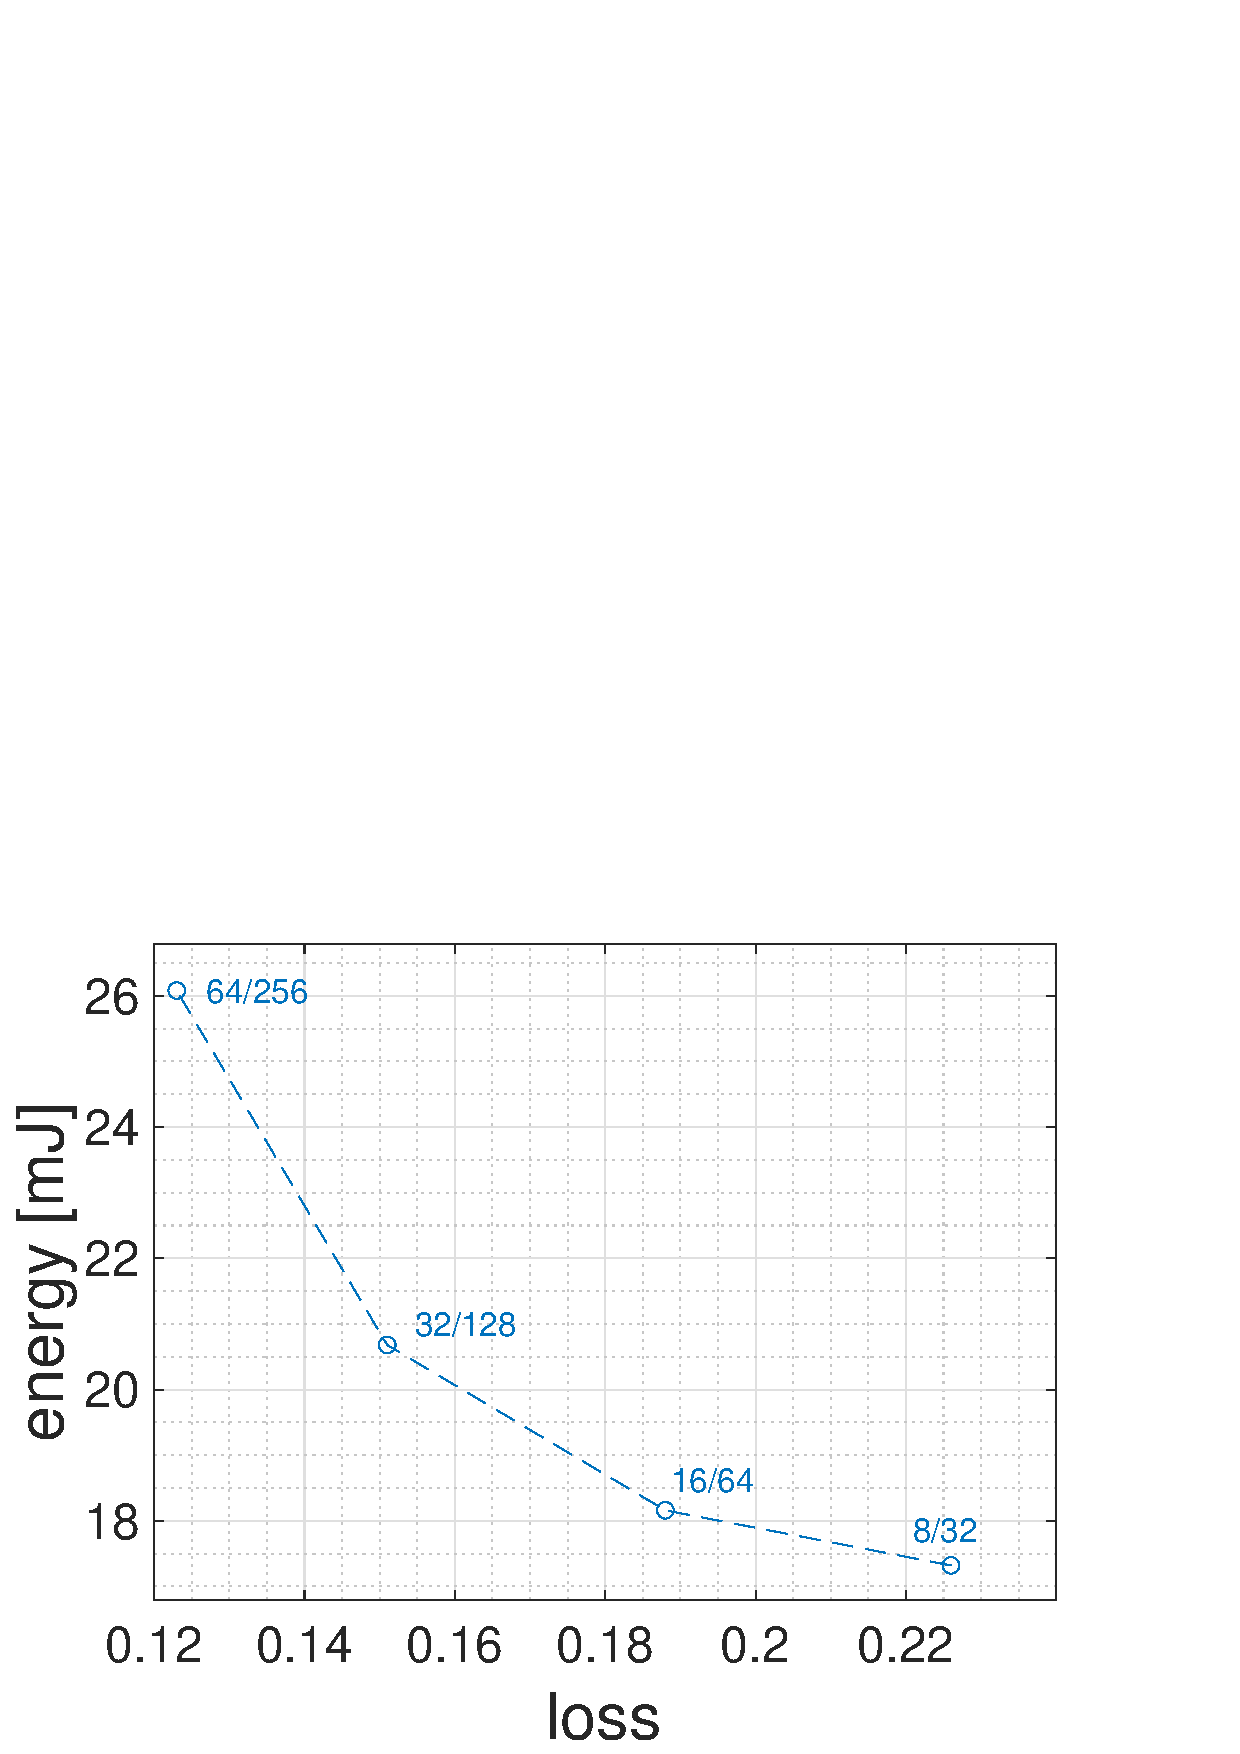
\includegraphics[width=\textwidth]{figure/lstm_energy_loss.pdf}
        \caption{consumo di energia vs. loss}
        \label{fig:performance-lstm-hexi:lstm-energy-loss}
    \end{subfigure}
    \begin{subfigure}{.45\textwidth}
        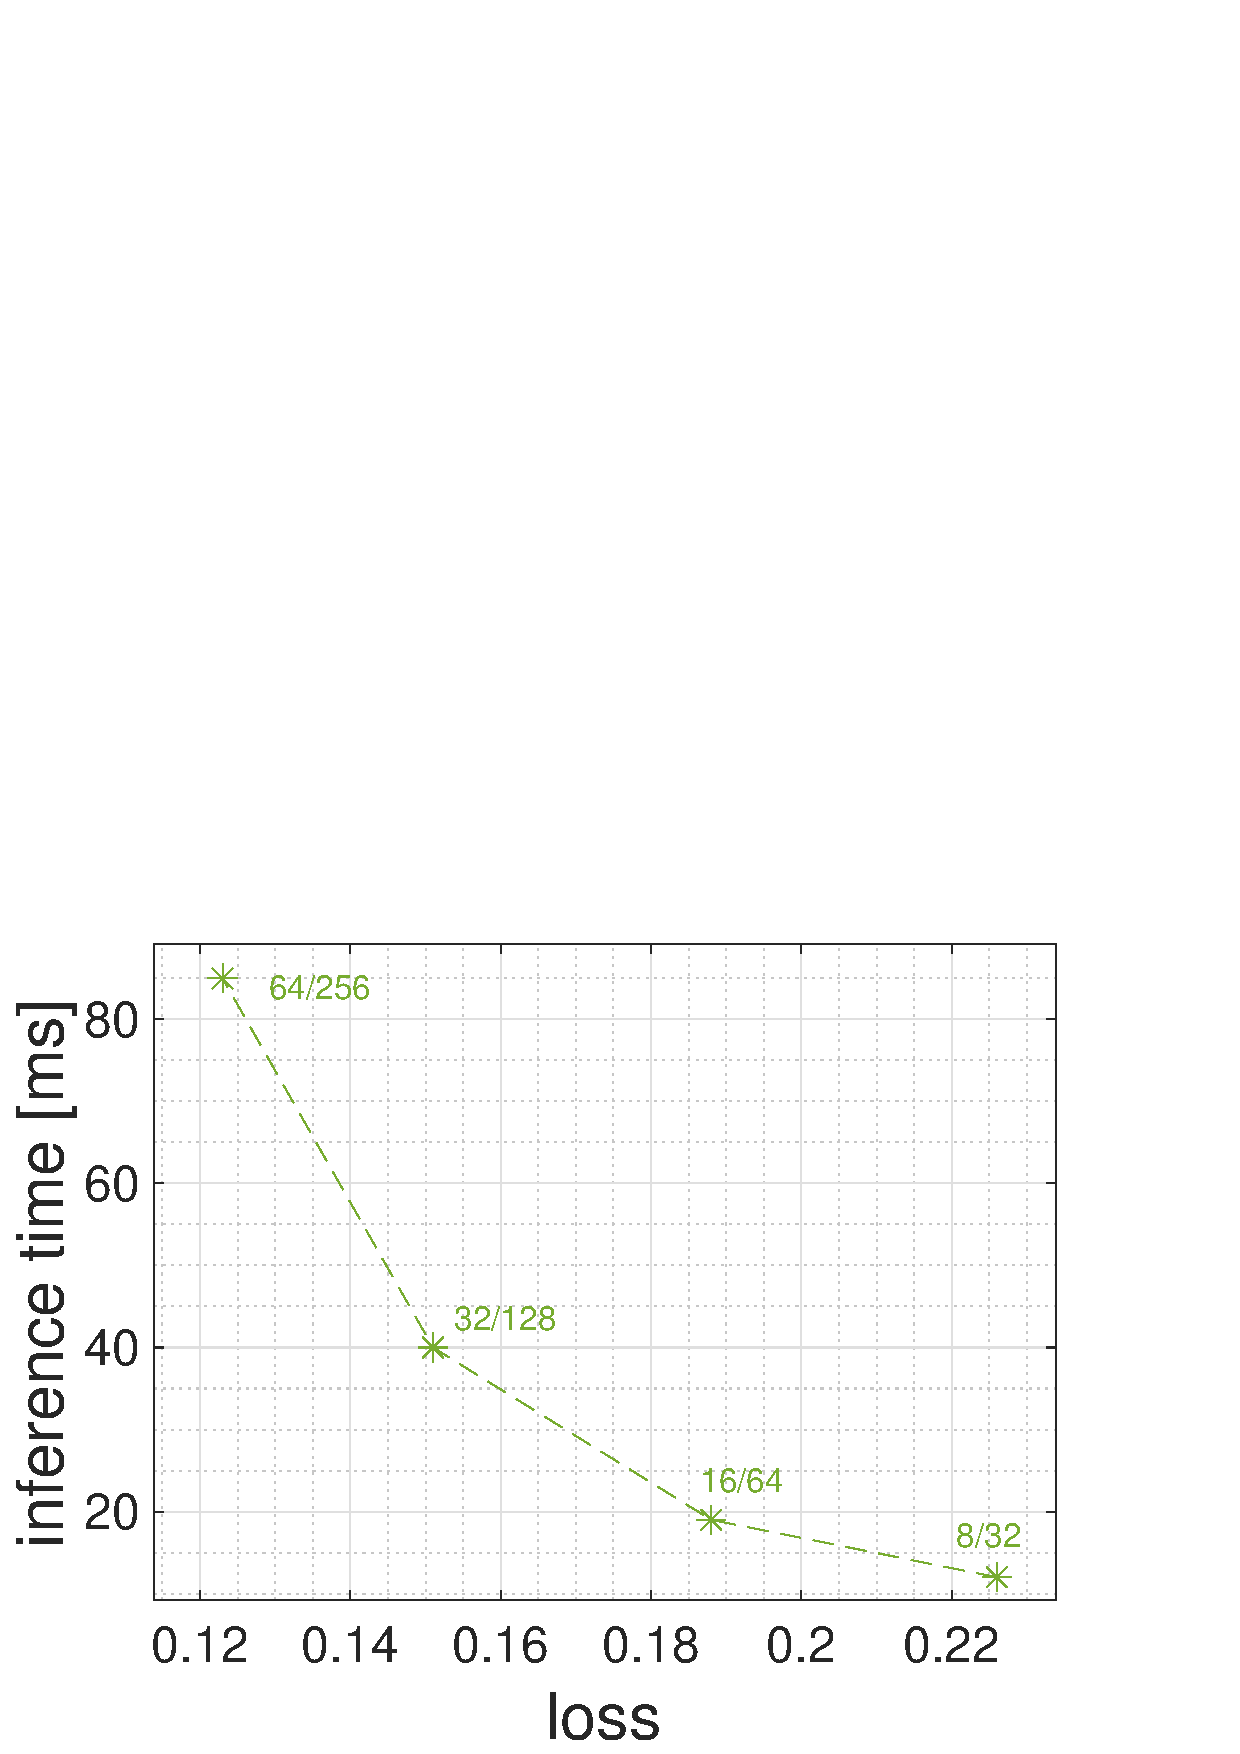
\includegraphics[width=\textwidth]{figure/lstm_time_loss.pdf}
        \caption{tempo d'inferenza vs. loss}
        \label{fig:performance-lstm-hexi:lstm-time-loss}
    \end{subfigure}
    \begin{subfigure}{.45\textwidth}
        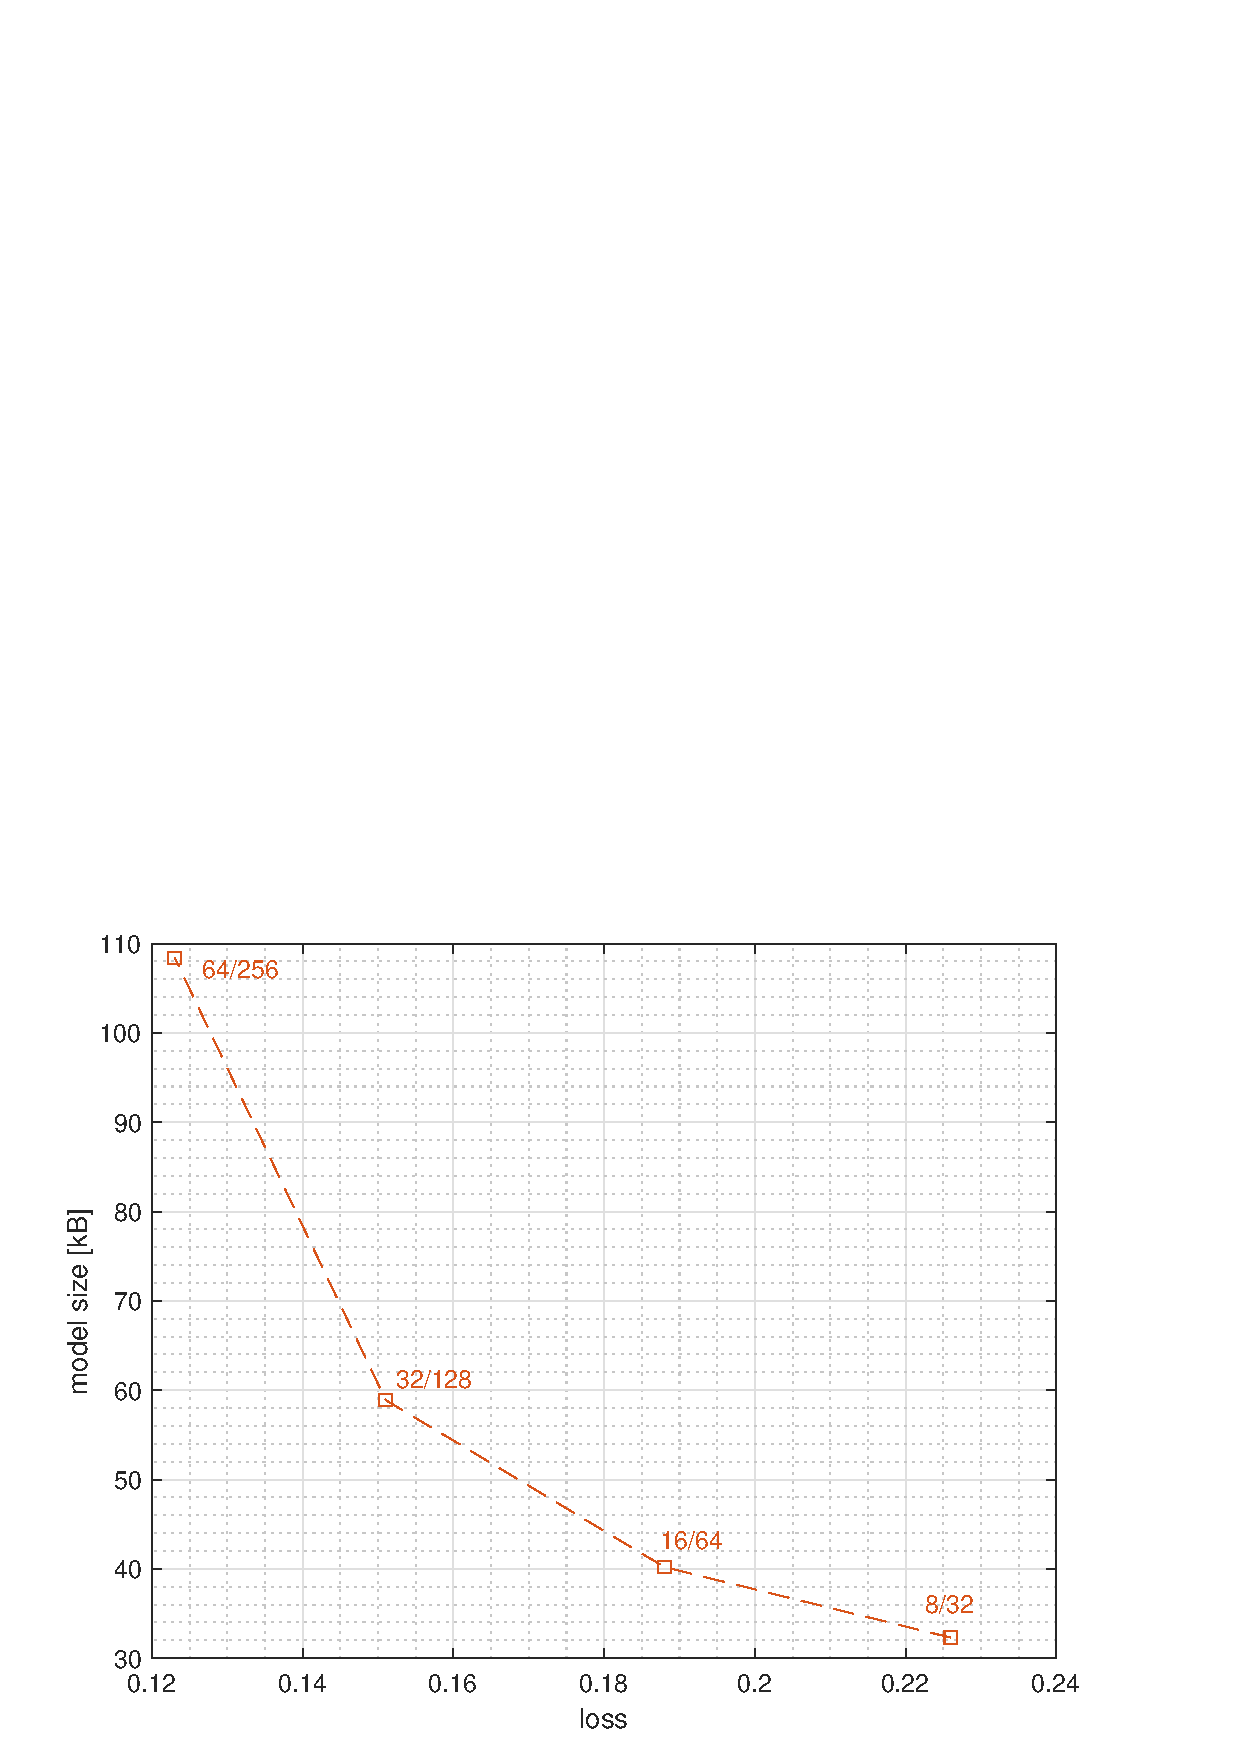
\includegraphics[width=\textwidth]{figure/lstm_size_loss.pdf}
        \caption{dimensione modello vs. loss}
        \label{fig:performance-lstm-hexi:lstm-size-loss}
    \end{subfigure}
    \caption{Grafici prodotti dal modello LSTM confrontando consumo d'energia(\subref{fig:performance-lstm-hexi:lstm-energy-loss}), tempo d'inferenza(\subref{fig:performance-lstm-hexi:lstm-time-loss}) e dimensione modello(\subref{fig:performance-lstm-hexi:lstm-size-loss}) con la loss.}
    \label{fig:performance-lstm-hexi}
\end{figure}

\section{Sviluppo dell'applicazione}
\label{sec:sviluppo-dell-applicazione}

In questa sezione presentiamo lo sviluppo di un'applicazione nativa per lo smartwatch HEXIWEAR. Dopo aver eseguito tutti gli esperimenti sui modelli di machine learning e di deep learning implementati sia su PC che sullo smartwatch abbiamo deciso di sviluppare un'applicazione per l'HEXIWEAR che metta in pratica quanto scoperto in questa tesi ad un contesto comune e più utile per tutti gli utenti. 

L'applicazione sviluppata ha lo scopo di conteggiare il numero di attività di lavaggio e di sanificazione della mani compiute da un utente nell'arco di una giornata; per fare questo raccoglie in maniera continua i valori non elaborati dai sensori di accelerometro e giroscopio ed utilizza uno dei modelli di machine learning visti precedentemente per classificare l'attività svolta. 

L'applicazione nativa è stata sviluppata interamente in C/C++ facendo uso delle API messe a disposizione dal sistema operativo real-time MbedOS; in particolare il processo di build è stato gestito della nuova toolchain CLI \textit{mbed-tools}\cite{mbedtools}, il quale automatizza la fase di building e di flash dell'applicazione e controlla tutti gli aspetti del progetto come rilevare automaticamente i dispositivi embedded connessi o mantenere aggiornate tutte le librerie esterne.

Nell'applicazione sono state utilizzate quattro librerie esterne: le librerie \textit{hexiwear\_FXAS21002}\cite{fxas21002} e \textit{hexiwear\_FXOS8700}\cite{fxos87700} hanno lo scopo di controllare gli omonimi sensori integrati di accelerometro e giroscopio leggendo i loro valori ad una frequenza di 100Hz. La libreria \textit{hexiwear\_KW40Z}\cite{kw40z} consente l'accesso alle funzionalità di Bluetooth Low Energy del micro-processore KW40Z, anche se non è questo il motivo per qui l'abbiamo scelta; infatti questo processore è responsabile anche della gestione di tutti gli eventi provenienti dai bottoni capacitivi posti sulla parte frontale del dispositivo. Infine l'ultima libreria utilizzata è \textit{oled\_ssd1351}\cite{ssd1351} che ha lo scopo di pilotare il display OLED presente sullo smartwatch; a differenza delle altre librerie, create e mantenute dal team di sviluppo dell'HEXIWEAR, questa è stata creata quasi da zero da noi partendo dalla versione ufficiale modificandola pesantemente per adeguarla alle nostre esigenze e risolvere alcuni fastidiosi bug.

\begin{figure}[!htb]
    \centering
    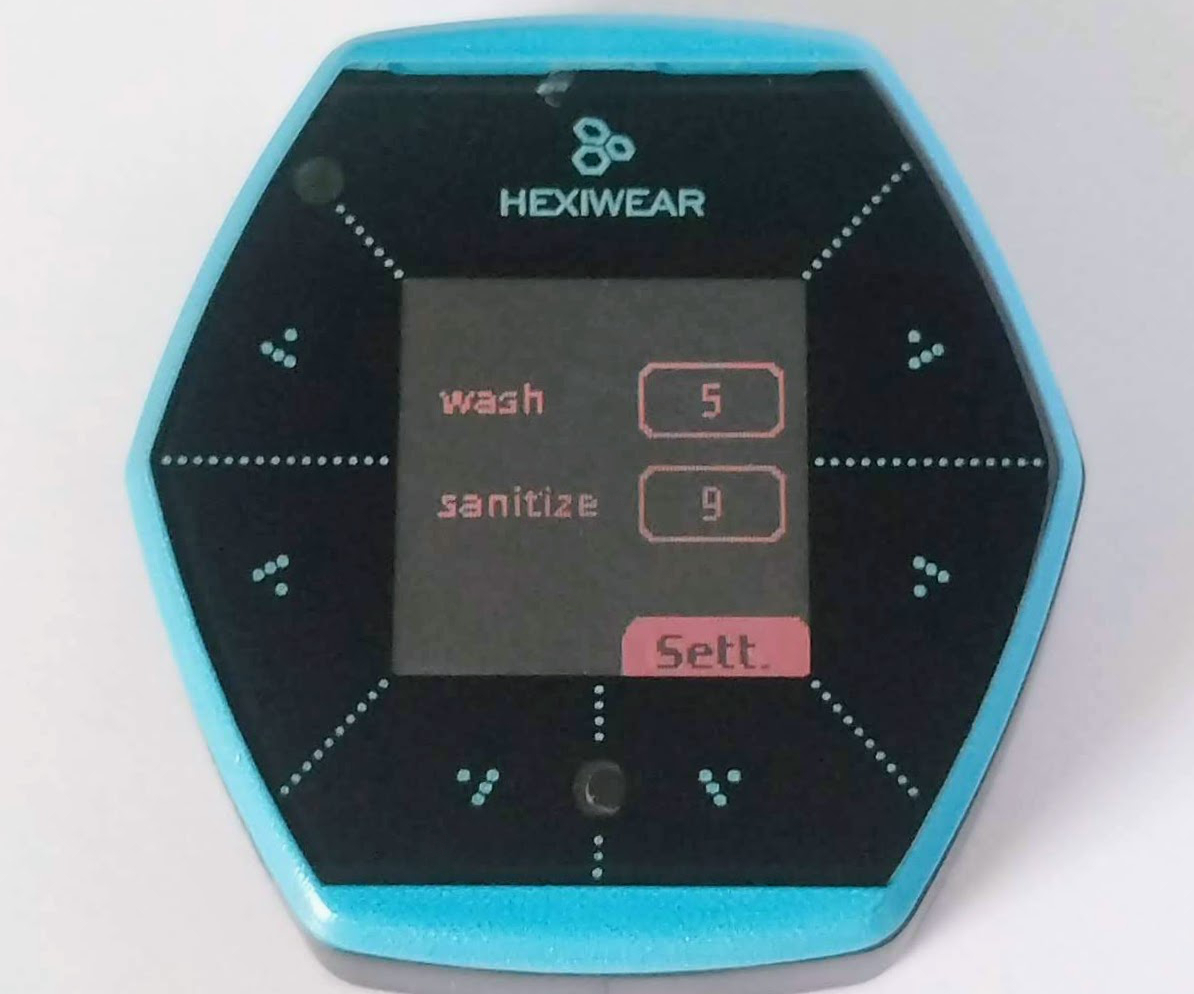
\includegraphics[width=.4\textwidth]{figure/hexiwear-app.jpg}
    \caption{Schermata principale dell'applicazione di monitoraggio delle attività sviluppata per l'HEXIWEAR.}
    \label{fig:hexiwear-app}
\end{figure}

In Figura \ref{fig:hexiwear-app} possiamo vedere la schermata principale dell'applicazione in esecuzione direttamente sul dispositivo HEXIWEAR; il design è semplice, composto da due soli contatori: uno per i lavaggi delle mani ed uno per le sanificazioni. Premendo il pulsante \textit{Settings} saremo portati nella pagina delle impostazioni, nella quale possiamo resettare i contatori a fine giornata.

Per il rilevamento delle attività l'applicazione fa uso del modello di deep learning LSTM presentato nella Sezione \ref{ssec:selezione-dei-parametri-di-lstm-hexi} con i parametri interni settati a 64 unità per il modulo LSTM e 256 neuroni per il primo livello densamente connesso. Si è scelto di utilizzare questa tipologia di rete poiché risulta essere la più prestante in termini delle metriche di accuratezza (tutte le metriche superano l'87\%); inoltre, anche se il tempo d'inferenza e la memoria utilizzata sono maggiori rispetto ai modelli SVM, il consumo d'energia è molto inferiore che, in definitiva, questo parametro non è da trascurare quando si parla di applicazioni embedded o indossabili che hanno bisogno di una lunga durata della batteria.
\chapter{Conclusioni}
\label{cap:conclusioni}

In questa tesi è stata condotta una ricerca estensiva volta a studiare l'abilità dei sistemi di machine learning nel distinguere le attività di lavaggio e sanificazione delle mani di gran parte della popolazione utilizzando strumenti di misurazione non invasivi come i comuni smartwatch reperibili commercialmente. In particolare ci siamo concentrati sul riconoscimento dei gesti di lavaggio partendo da dati non strutturati, ovvero prodotti da utenti non istruiti sulla corretta maniera in cui lavare o sanificare le mani i quali sono stati lasciati liberi di usare il loro metodo di lavaggio abituale. Durante la ricerca siamo giunti alla creazione di un dataset personalizzato utilizzando una IMU posizionata sul polso dominante per raccogliere svariate ore di dati durante attività di vita reale dai diversi soggetti.

Il dataset costruito ad hoc, assieme ad un dataset DLA disponibile pubblicamente sono stati utilizzati per addestrare i diversi modelli di machine learning e di deep learning durante una serie di esperimenti condotti sia su ambiente PC che direttamente sullo smartwatch scelto: l'HEXIWEAR. Questi esperimenti hanno permesso di valutare le performance delle diverse tipologie di modelli su un ambiente dalle risorse pressoché illimitate, quello PC, ma anche su uno smartwatch le cui risorse sono altamente limitate, sia in termini di memoria che di potenza di calcolo e di durata della batteria. Dalla ricerca è emerso che in ambente PC e con il dataset costruito ad hoc i modelli hanno prodotto metriche di accuratezza con valori superiori al 93\%, mentre sul dispositivo HEXIWEAR, a causa delle minori risorse, le performance sono scese attorno all'87\%; ciò dimostra che le operazioni di riconoscimento e monitoraggio di queste attività tramite dati inerziali raccolti dal polso dell'utente mediante un comune smartwatch sono totalmente fattibili e producono ottimi risultati, in linea con gli studi sul riconoscimento delle altre tipologie di attività umane, come la corsa e la camminata.

Nell'ultima parte di questa tesi abbiamo presentato lo sviluppo di un'applicazione nativa per lo smartwatch HEXIWEAR con lo scopo di monitorare costantemente l'igiene delle mani dell'utente che lo indossa; per fare questo i sensori di accelerometro e giroscopio sono campionati costantemente ed il modello di deep learning LSTM è usato per classificare le corrette attività aggiornando l'interfaccia grafica.

Uno dei potenziali sviluppi futuri di questo lavoro consiste nell'approfondire la ricerca svolta in tutti gli ambiti, in particolare ampliando il dataset costruito ad hoc raccogliendo ancora più ore di dati da un maggior numero di soggetti di genere ed età diversi; in questo modo si va a creare un dataset pubblico di ottima qualità specifico per le misurazioni delle attività non strutturate di lavaggio e sanificazione delle mani, che, dalle nostre ricerche, non sembra ancora esistere.
La ricerca può essere ampliata anche nell'ambito dei sistemi di machine learning svolgendo molti più test. 
Infine un’ultima area di miglioramento è la qualità dei modelli portati sullo smartwatch; a causa delle grandi limitazioni in termini di memoria siamo stati costretti a ridurre severamente la dimensione dei modelli eseguiti sull'HEXIWEAR. Uno sviluppo futuro prevede sicuramente l’analisi dei dispositivi più performanti in grado di eseguire gli stessi modelli studiati nell’ambiente PC.
%\include{sorgenti/cap_6}
%\include{sorgenti/cap_7}
%\include{sorgenti/cap_8}

\appendix
% \include{sorgenti/app_a}
\begin{thebibliography}{99}
	\bibitem{santarpia2020aerosol}Santarpia, J., Rivera, D., Herrera, V., Morwitzer, M., Creager, H., Santarpia, G., Crown, K., Brett-Major, D., Schnaubelt, E., Broadhurst, M. \& Others Aerosol and surface contamination of SARS-CoV-2 observed in quarantine and isolation care. {\em Scientific Reports}. \textbf{10}, 1-8 (2020)
    \bibitem{wang2020accurate}Wang, C., Sarsenbayeva, Z., Chen, X., Dingler, T., Goncalves, J., Kostakos, V. \& Others Accurate measurement of handwash quality using sensor armbands: Instrument validation study. {\em JMIR MHealth And UHealth}. \textbf{8}, e17001 (2020)
    \bibitem{zhang2013human}Zhang, M. \& Sawchuk, A. Human daily activity recognition with sparse representation using wearable sensors. {\em IEEE Journal Of Biomedical And Health Informatics}. \textbf{17}, 553-560 (2013)
    \bibitem{sztyler2016body}Sztyler, T. \& Stuckenschmidt, H. On-body localization of wearable devices: An investigation of position-aware activity recognition. {\em 2016 IEEE International Conference On Pervasive Computing And Communications (PerCom)}. pp. 1-9 (2016)
    \bibitem{sztyler2017position}Sztyler, T., Stuckenschmidt, H. \& Petrich, W. Position-aware activity recognition with wearable devices. {\em Pervasive And Mobile Computing}. \textbf{38} pp. 281-295 (2017)
    \bibitem{bhat2018online}Bhat, G., Deb, R., Chaurasia, V., Shill, H. \& Ogras, U. Online human activity recognition using low-power wearable devices. {\em 2018 IEEE/ACM International Conference On Computer-Aided Design (ICCAD)}. pp. 1-8 (2018)
    \bibitem{koping2018general}Köping, L., Shirahama, K. \& Grzegorzek, M. A general framework for sensor-based human activity recognition. {\em Computers In Biology And Medicine}. \textbf{95} pp. 248-260 (2018)
    \bibitem{lattanzi2022exploring}Lattanzi, E., Donati, M. \& Freschi, V. Exploring Artificial Neural Networks Efficiency in Tiny Wearable Devices for Human Activity Recognition. {\em Sensors}. \textbf{22}, 2637 (2022)
    \bibitem{cheng2010active}Cheng, J., Amft, O. \& Lukowicz, P. Active capacitive sensing: Exploring a new wearable sensing modality for activity recognition. {\em International Conference On Pervasive Computing}. pp. 319-336 (2010)
    \bibitem{singh2017convolutional}Singh, D., Merdivan, E., Hanke, S., Kropf, J., Geist, M. \& Holzinger, A. Convolutional and recurrent neural networks for activity recognition in smart environment. {\em Towards Integrative Machine Learning And Knowledge Extraction}. pp. 194-205 (2017)
    \bibitem{hassan2018robust}Hassan, M., Uddin, M., Mohamed, A. \& Almogren, A. A robust human activity recognition system using smartphone sensors and deep learning. {\em Future Generation Computer Systems}. \textbf{81} pp. 307-313 (2018)
    \bibitem{hou2020study}Hou, C. A study on IMU-based human activity recognition using deep learning and traditional machine learning. {\em 2020 5th International Conference On Computer And Communication Systems (ICCCS)}. pp. 225-234 (2020)
    \bibitem{muller2021ten}Muller, H., Mayrhofer, M., Van Veen, E. \& Holzinger, A. The ten commandments of ethical medical AI. {\em Computer}. \textbf{54}, 119-123 (2021)
    \bibitem{zhong2020multi}Zhong, C., Reibman, A., Mina, H. \& Deering, A. Multi-view hand-hygiene recognition for food safety. {\em Journal Of Imaging}. \textbf{6}, 120 (2020)
    \bibitem{yue2021intelligent}Yue, Z., Wang, F. \& Liu, Z. An intelligent hand-washing monitoring platform based on gesture recognition technology. {\em 2021 China Automation Congress (CAC)}. pp. 940-944 (2021)
    \bibitem{galluzzi2015hand}Galluzzi, V., Herman, T. \& Polgreen, P. Hand hygiene duration and technique recognition using wrist-worn sensors. {\em Proceedings Of The 14th International Conference On Information Processing In Sensor Networks}. pp. 106-117 (2015)
    \bibitem{bal2017system}Bal, M. \& Abrishambaf, R. A system for monitoring hand hygiene compliance based-on Internet-of-Things. {\em 2017 IEEE International Conference On Industrial Technology (ICIT)}. pp. 1348-1353 (2017)
    \bibitem{li2018wristwash}Li, H., Chawla, S., Li, R., Jain, S., Abowd, G., Starner, T., Zhang, C. \& Plötz, T. Wristwash: towards automatic handwashing assessment using a wrist-worn device. {\em Proceedings Of The 2018 ACM International Symposium On Wearable Computers}. pp. 132-139 (2018)
    \bibitem{jain2018gender}Jain, A. \& Kanhangad, V. Gender classification in smartphones using gait information. {\em Expert Systems With Applications}. \textbf{93} pp. 257-266 (2018)
    \bibitem{van2019systematic}Van Hamme, T., Garofalo, G., Argones Rúa, E., Preuveneers, D. \& Joosen, W. A systematic comparison of age and gender prediction on imu sensor-based gait traces. {\em Sensors}. \textbf{19}, 2945 (2019)
    \bibitem{mondol2015harmony}Mondol, M. \& Stankovic, J. Harmony: A hand wash monitoring and reminder system using smart watches. {\em Proceedings Of The 12th EAI International Conference On Mobile And Ubiquitous Systems: Computing, Networking And Services On 12th EAI International Conference On Mobile And Ubiquitous Systems: Computing, Networking And Services}. pp. 11-20 (2015)
    \bibitem{mondol2020hawad}Mondol, M. \& Stankovic, J. HAWAD: Hand washing detection using wrist wearable inertial sensors. {\em 2020 16th International Conference On Distributed Computing In Sensor Systems (DCOSS)}. pp. 11-18 (2020)
    \bibitem{banerjee2020hand}Banerjee, A., Amperyani, V. \& Gupta, S. Hand hygiene compliance checking system with explainable feedback. {\em Proceedings Of The 6th ACM Workshop On Wearable Systems And Applications}. pp. 34-36 (2020)
    \bibitem{samyoun2021iwash}Samyoun, S., Shubha, S., Mondol, M. \& Stankovic, J. iWash: A smartwatch handwashing quality assessment and reminder system with real-time feedback in the context of infectious disease. {\em Smart Health}. \textbf{19} pp. 100171 (2021)
    \bibitem{fagert2022clean}Fagert, J., Bonde, A., Srinidhi, S., Hamilton, S., Zhang, P. \& Noh, H. Clean Vibes: Hand Washing Monitoring Using Structural Vibration Sensing. {\em ACM Transactions On Computing For Healthcare}. (2022)
    \bibitem{lattanzi2022unstructured}Lattanzi, E., Calisti, L. \& Freschi, V. Unstructured Handwashing Recognition using Smartwatch to Reduce Contact Transmission of Pathogens. {\em IEEE Access}. (2022)
    \bibitem{leotta2021daily}Leotta, M., Fasciglione, A. \& Verri, A. Daily living activity recognition using wearable devices: A features-rich dataset and a novel approach. {\em International Conference On Pattern Recognition}. pp. 171-187 (2021)
    \bibitem{shimmer}Shimmer Shimmer3 IMU unit. , https://shimmersensing.com/, Accessed 20/08/2022
    \bibitem{wang2015imaging}Wang, Z. \& Oates, T. Imaging time-series to improve classification and imputation. {\em Twenty-Fourth International Joint Conference On Artificial Intelligence}. (2015)
\end{thebibliography}

\ringraziamenti
Vorrei ringraziare di cuore tutte le persone che mi hanno supportato durante questo lavoro di tesi; un ringraziamento speciale va al Prof. Lattanzi per i suoi indispensabili consigli, per le conoscenze trasmesse e per la sua infinita disponibilità in ogni passo della realizzazione dell’elaborato.
Ringrazio infinitamente la mia famiglia, senza i loro insegnamenti e senza il loro supporto, questo lavoro di tesi non esisterebbe nemmeno.
Ringrazio tutti i miei amici per essere stati sempre presenti anche durante quest’ultima fase del mio percorso di studi.

\end{document}
